\section{Numerical examples} 
\label{Sec2:resultsDisc}
We start by investigating the pollution effect for the scattering problem on a rigid sphere, and then continue with the acoustic structure interaction (ASI) problem on the spherical shell. Rigid scattering on a sphere and elastic scattering on a spherical shell are often used to verify the methods because both cases admits analytic solutions. The latter case is the only known problem which admits such an analytic solution for the ASI scattering problem in 3D, and is thus especially valuable. Moreover, these cases has been used as a benchmark example for many methods and one is then able to compare the performance of each method on this problem.

The multipole layers for the infinite elements will be placed at $r_n=nr_{\mathrm{a}}$ for $n=1,\dots,N$ (this is suggested by Burnett in~\cite{Burnett1994atd}). Moreover, unless otherwise stated, we shall use the PGU formulation by default for the infinite elements.

\subsection{Plane wave scattered by a rigid sphere}
Let the plane wave\footnote{We here use the spherical coordinate system where $r\in[0,\infty)$ is the radius, $\vartheta\in[0,\pi]$ is the polar angle and $\varphi\in[0,2\pi)$ is the asimuth angle satisfying the relations
\begin{equation*}
	x = r\sin\vartheta\cos\varphi,\quad y = r\sin\vartheta\sin\varphi,\quad z = r\cos\vartheta.
\end{equation*}
} (with $\vec{k}=[0, 0, k]^\transpose$)
\begin{equation*}
	p_{\textrm{inc}}(r,\vartheta) = P_{\mathrm{inc}}\euler^{\imag kz} = P_{\mathrm{inc}}\euler^{\imag kr\cos\vartheta}
\end{equation*}
be scattered on a sphere with radius $R=0.5$. That is, we send the wave along the $z$-axis. The resulting scattered wave is then\footnote{Here, $P_n(x)$ denotes the $n^{\mathrm{th}}$ Legendre polynomial and $j_n(x)$ denotes the $n^{\mathrm{th}}$ spherical Bessel function of first kind, and $h_n(x)$ denotes the $n^{\mathrm{th}}$ spherical Hankel function of the first kind.} (rigid scattering)
\begin{equation}\label{Eq2:rigidScattering_p}
	p_{\mathrm{rs}} (r,\vartheta) = -P_{\mathrm{inc}}\sum_{n=0}^\infty \imag^n (2n+1) P_n(\cos\vartheta)\frac{j_n'(kR)}{h_n'(kR)} h_n(kr).
\end{equation}
When computing the $H^1$-norm of the error we will also need the corresponding gradient, which in spherical coordinates is given by
\begin{align*}
	\nabla p_{\mathrm{rs}} (r,\vartheta) &= \pderiv{p_{\mathrm{rs}}}{r}\vec{e}_{\mathrm{r}} + \frac{1}{r}\pderiv{p_{\mathrm{rs}}}{\vartheta}\vec{e}_{\upvartheta} + \frac{1}{r\sin\vartheta}\pderiv{p_{\mathrm{rs}}}{\varphi}\vec{e}_{\upvarphi}\\
	&= -P_{\mathrm{inc}}\sum_{n=0}^\infty \imag^n (2n+1) \frac{j_n'(kR)}{h_n'(kR)} \left(P_n(\cos\vartheta)kh_n'(kr)\vec{e}_{\mathrm{r}} - \frac{\sin\vartheta}{r}P_n'(\cos\vartheta)h_n(kr)\vec{e}_{\upvartheta}\right)
\end{align*}
where the involved unit vectors in spherical coordinates are related to the Cartesian coordinates by
\begin{align*}
	\vec{e}_{\mathrm{r}} &= \sin\vartheta\cos\varphi\vec{e}_{\mathrm{x}} + \sin\vartheta\vec{e}_{\mathrm{y}} + \cos\vartheta\vec{e}_{\mathrm{z}}\\
	\vec{e}_{\upvartheta} &= \cos\vartheta\cos\varphi\vec{e}_{\mathrm{x}} + \cos\vartheta\sin\varphi\vec{e}_{\mathrm{y}} - \sin\vartheta\vec{e}_{\mathrm{z}}.
\end{align*}
For details of this solution see Ihlenburg~\cite[p. 28]{Ihlenburg1998fea}. Since this example has been used in~\cite{Gerdes1999otp} and~\cite{Simpson2014aib}, we may compare our results to the results found in these papers. We start by comparing the results found in~\cite{Simpson2014aib} by considering $k=2$ (low frequencies), and the construction of NURBS meshes illustrated in \Cref{Fig2:SphericalShellMeshes}. We send the incident wave along the $z$-axis (instead of the $x$-axis) and align the symmetry of the NURBS parametrization along the $y$-axis (instead of the $z$-axis). The results should obviously remain unchanged. We shall use $N=3$, which will practically neglect the error from the infinite element implementation on the coarse meshes considered. For low frequencies and the usage of the PGU formulation, it seems to be advantageous to set the artificial boundary very close to the surface of the sphere. We find the optimal radius to be around $r_{\mathrm{a}}=0.51$. When comparing with BEM, we typically have more liberty of adding degrees of freedom in the radial direction without destroying the fairness of the comparison. This is because the computational time of solving an BEM system of equations is higher than the corresponding IGA/IEM system of equations. However, it is very hard to compare the two methods without running both methods on the same computers. In~\Cref{Fig2:scatteringRigidSphereErrorNearField} we plot the absolute relative error in the modulus of the scattered field at $r=5$ (as was done in~\cite{Simpson2014aib}). Comparing with the results in~\cite{Simpson2014aib} we observe that BEM has the advantage on the coarsest mesh, but IGA/IEM produce the best results on finer meshes. 
%In~\Cref{Fig2:SphericalShellErrorMesh1}, \Cref{Fig2:SphericalShellErrorMesh2} and \Cref{Fig2:SphericalShellErrorMesh3} we visualize the error at the artificial boundary $\Gamma_{\mathrm{a}}$ both in the scalar field and the normed gradient field for mesh 1, 2 and 3, respectively. The gradient is used to evaluate far field points, so it is of interest to study this error as well. Interestingly, we observe larger errors in the gradient where the basis functions have lower continuity (which occurs at the mesh lines).
\begin{figure}
	\centering
	\begin{subfigure}{0.23\textwidth}
		\centering
		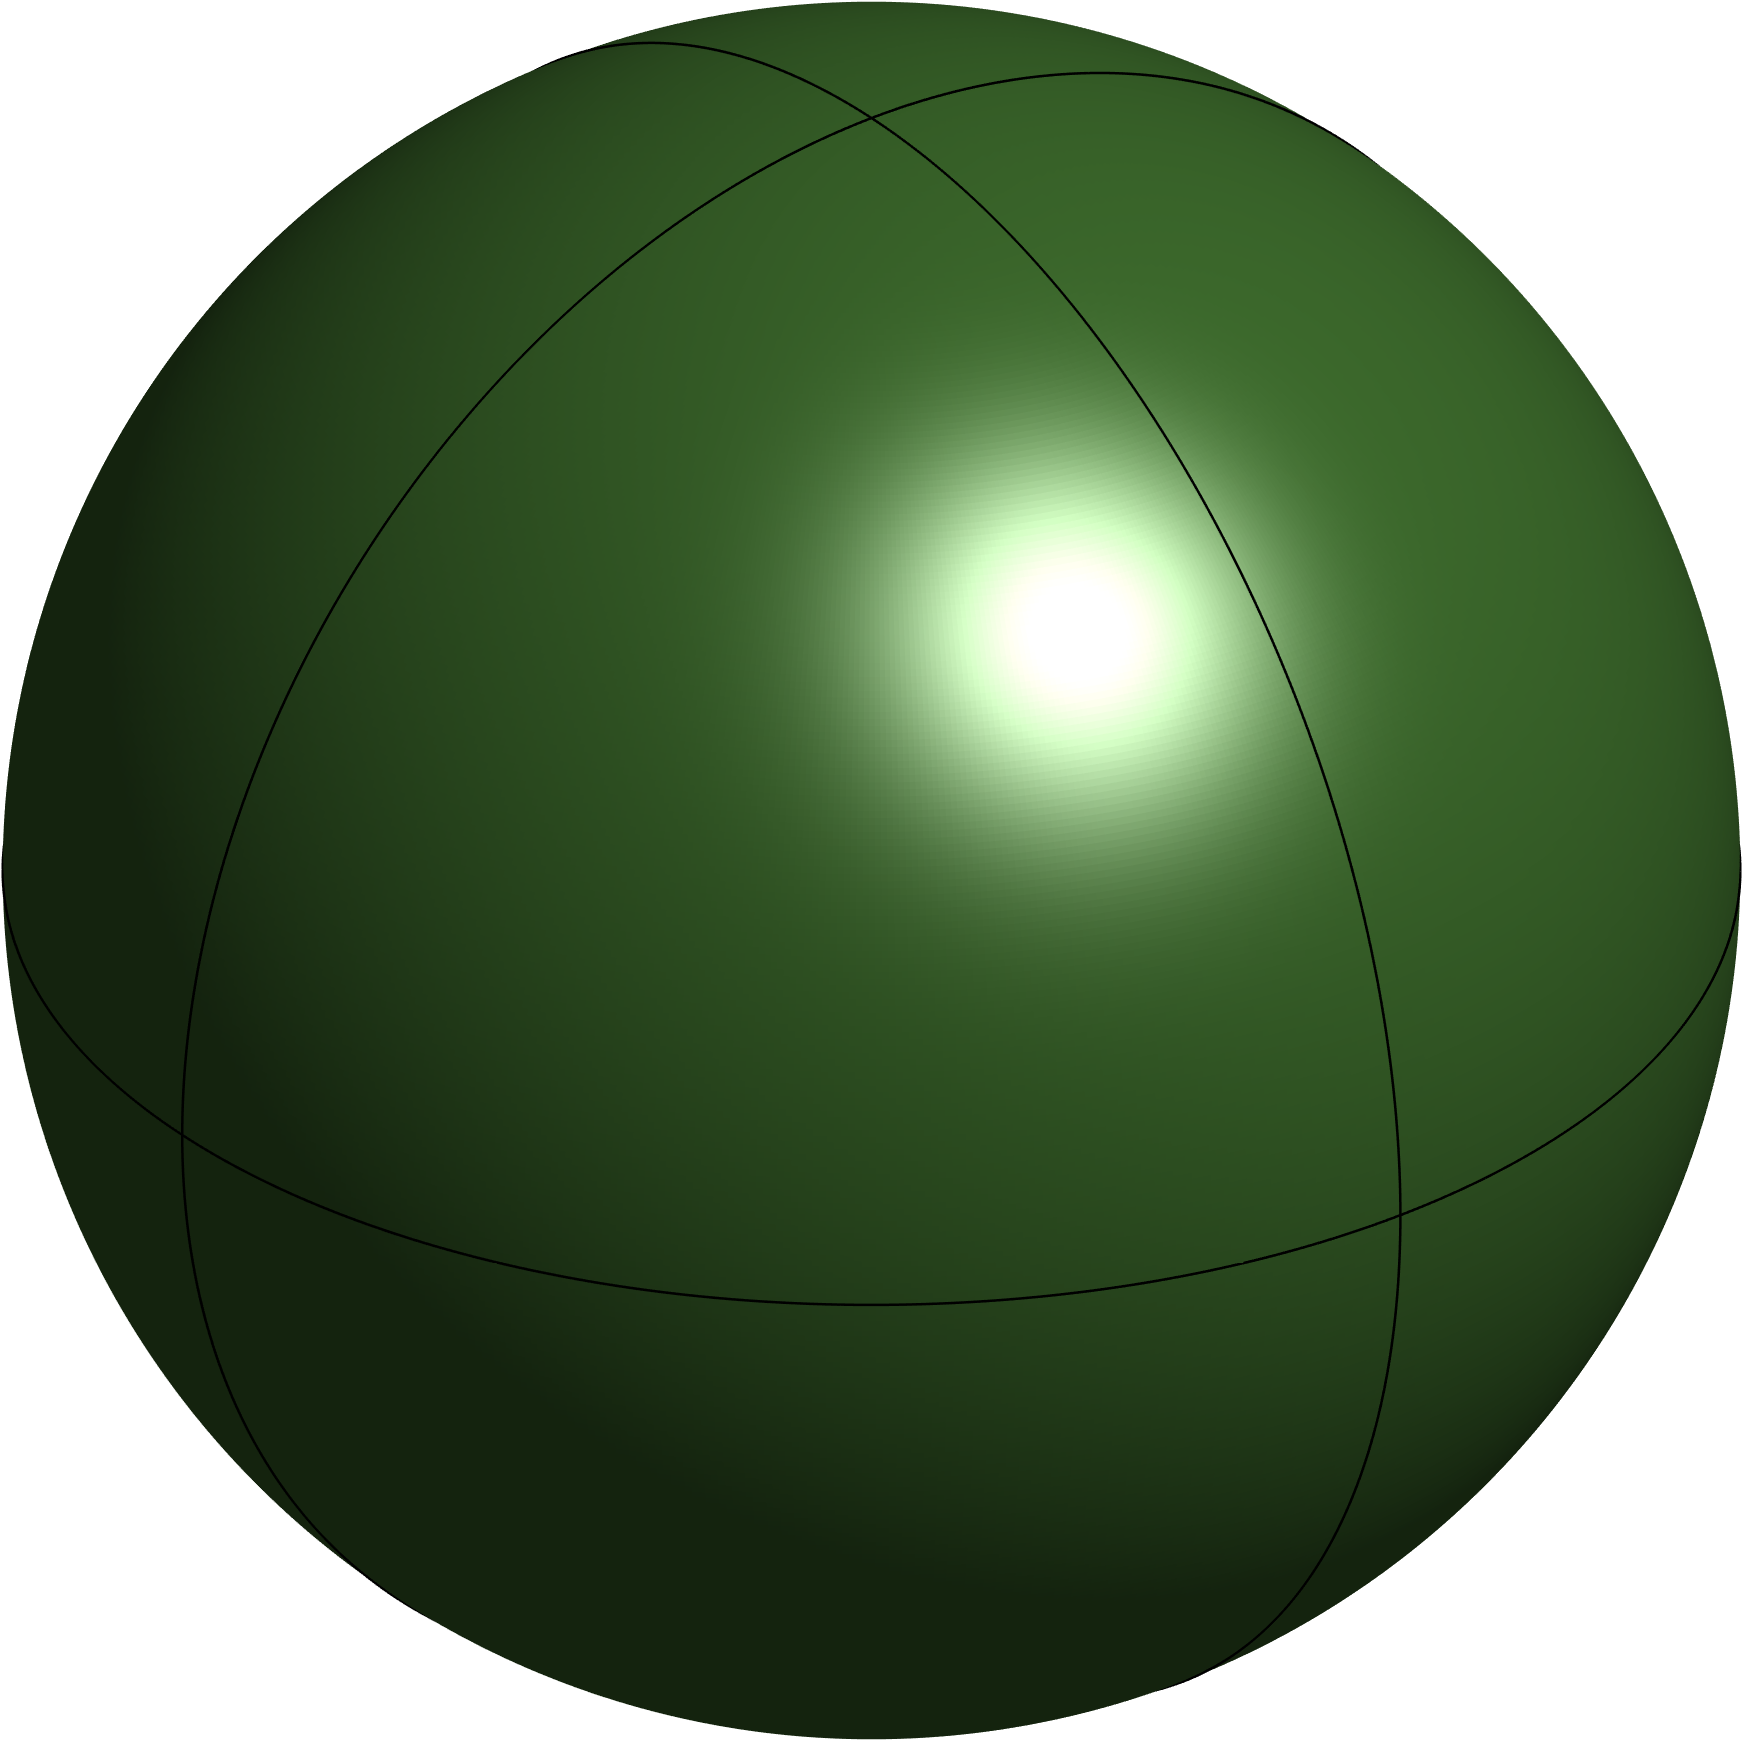
\includegraphics[width=\textwidth]{../../graphics/sphericalShell/sphericalShellMesh1_2_0}
		\caption{Mesh 1}
    \end{subfigure}
    ~
	\begin{subfigure}{0.23\textwidth}
		\centering
		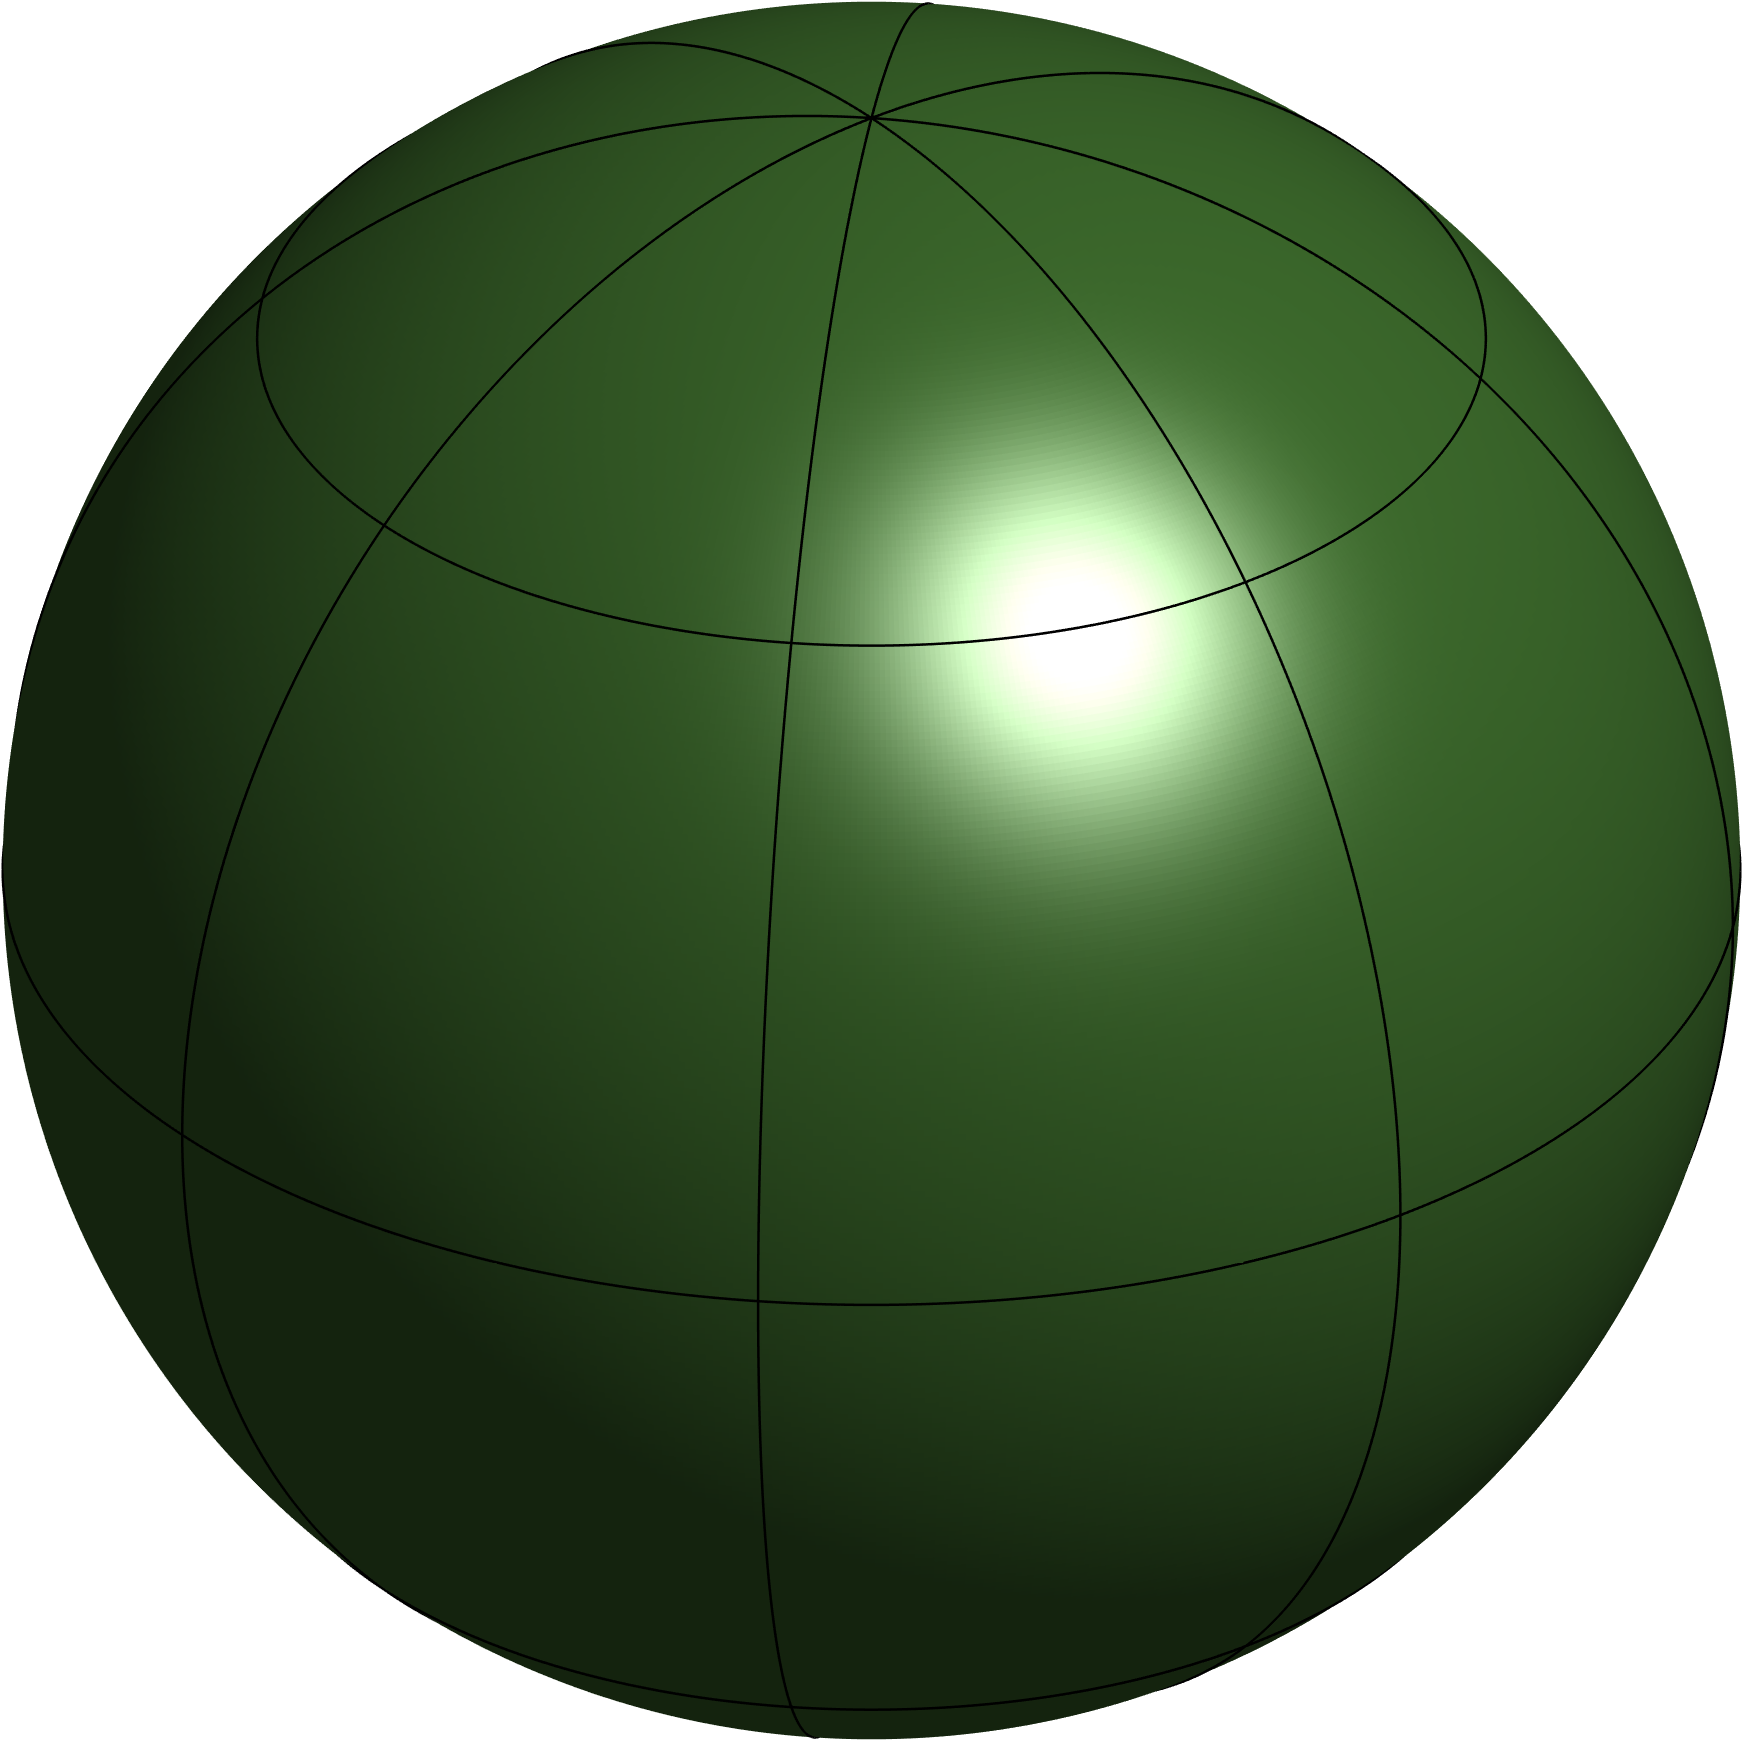
\includegraphics[width=\textwidth]{../../graphics/sphericalShell/sphericalShellMesh2_2_0}
		\caption{Mesh 2}
		\label{Fig2:SphericalShellMeshes2}
    \end{subfigure}
    ~
	\begin{subfigure}{0.23\textwidth}
		\centering
		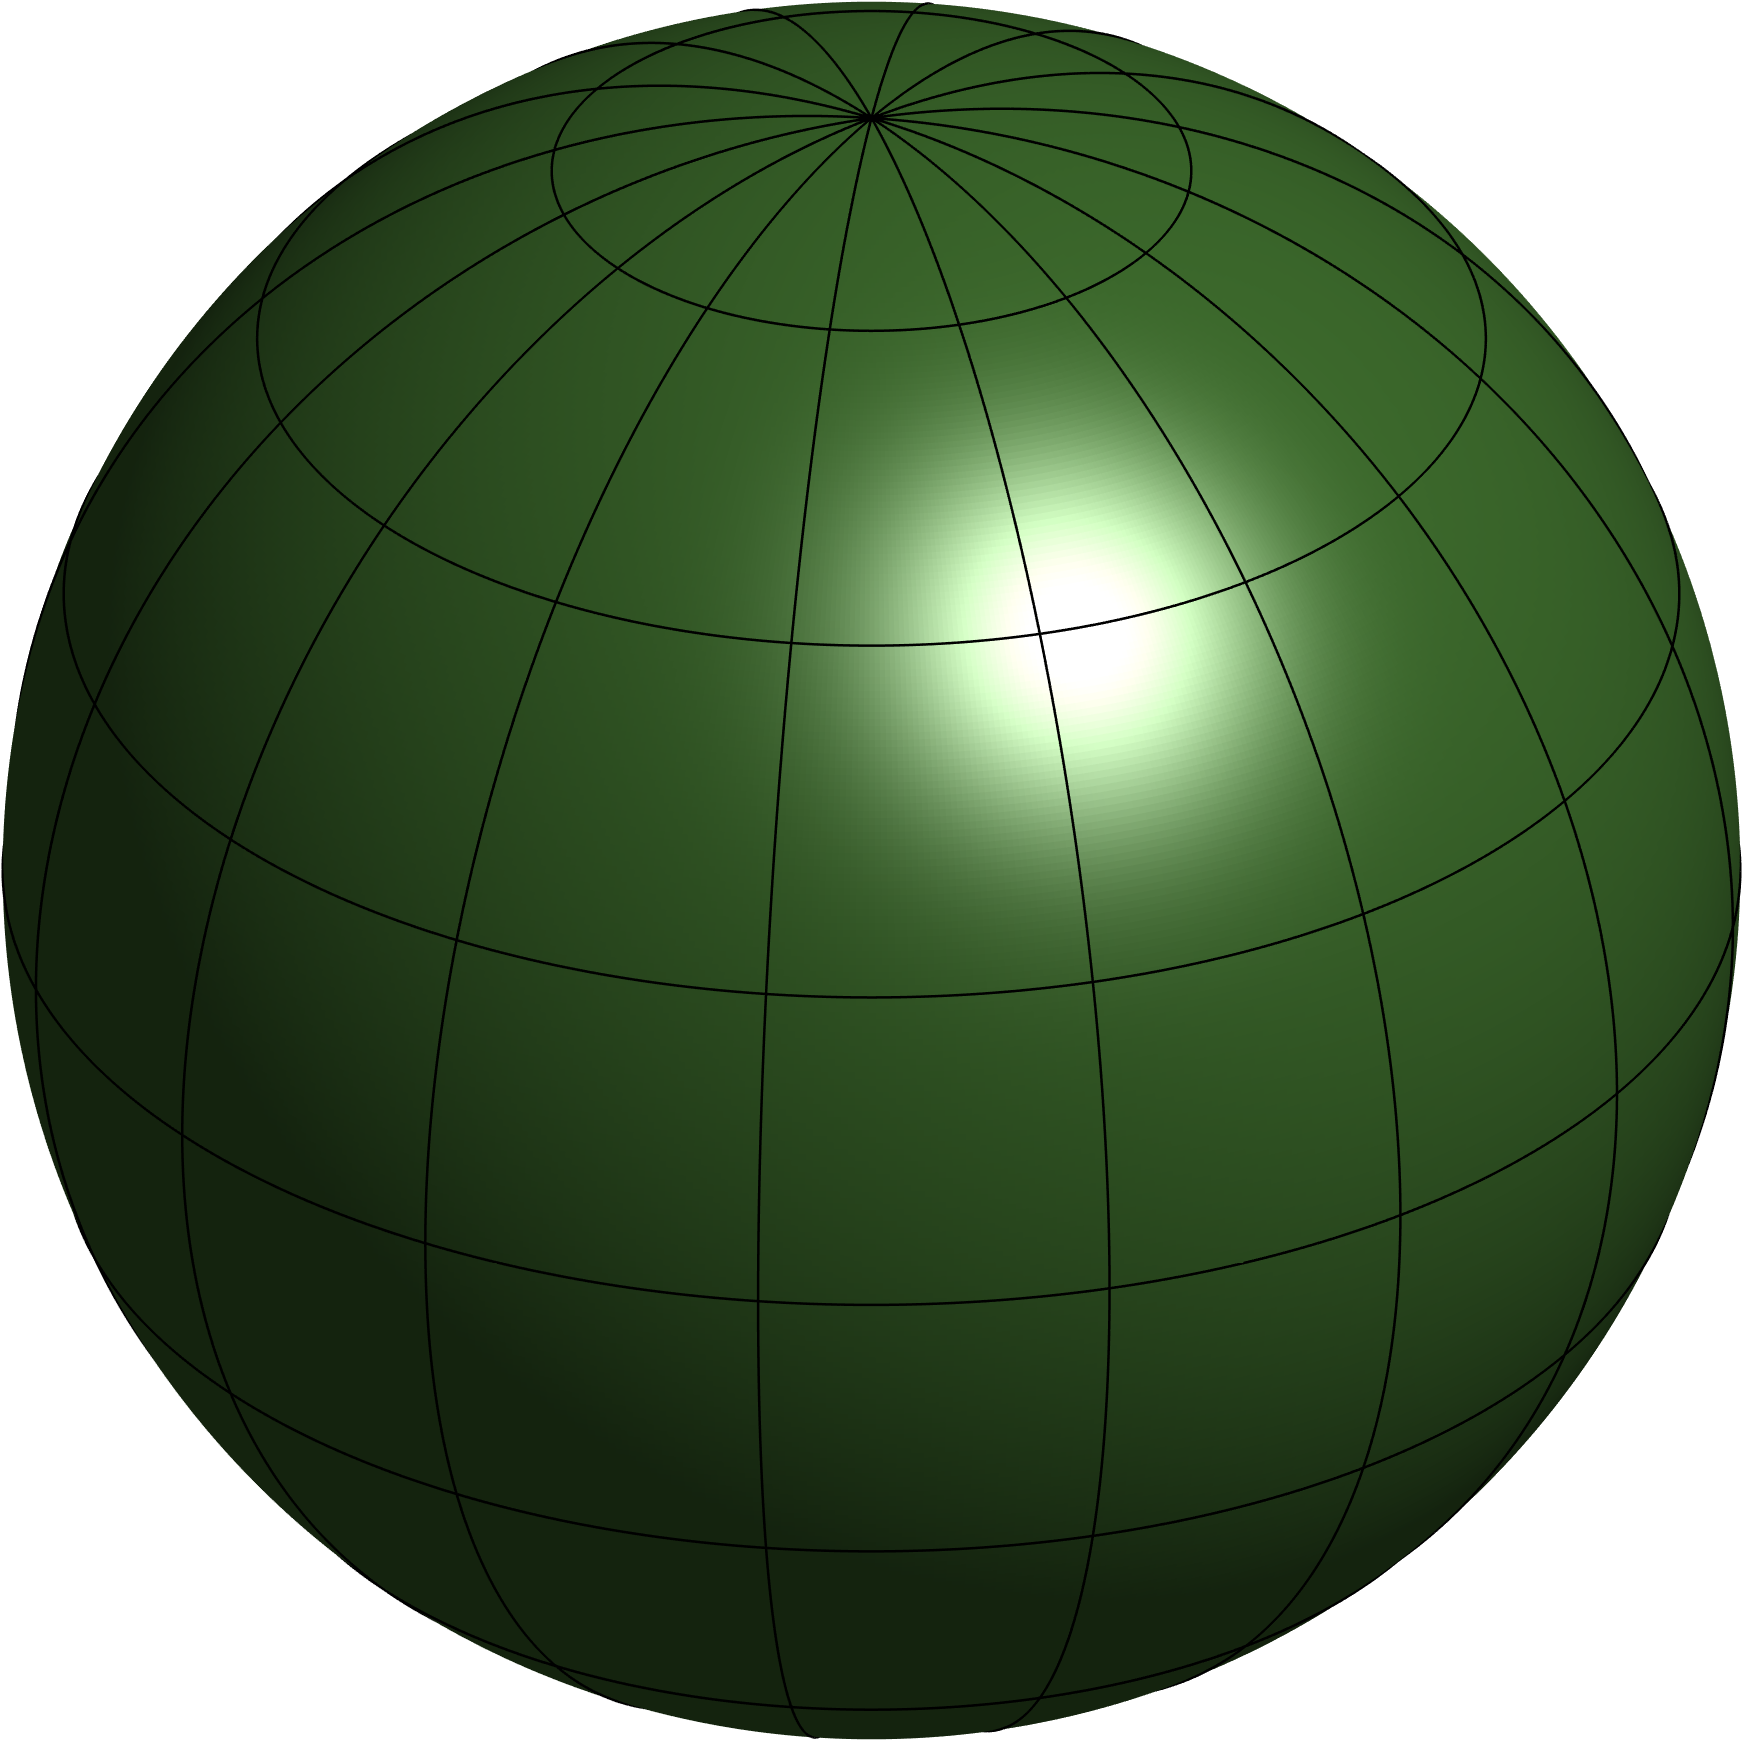
\includegraphics[width=\textwidth]{../../graphics/sphericalShell/sphericalShellMesh3_2_0}
		\caption{Mesh 3}
		\label{Fig2:SphericalShellMeshes3}
    \end{subfigure}
	\caption{\textbf{Plane wave scattered by a rigid sphere:} Meshes. The knot $\zeta=0.5$ has been inserted in $\Zeta$ for mesh 2 while the knots $\zeta = 0.25, 0.5, 0.75$ has been inserted in $\Zeta$ for mesh 3 (from the original mesh 1, with NURBS data found in \Cref{Sec2:NURBSdata}).}
	\label{Fig2:SphericalShellMeshes}
\end{figure}

\tikzsetnextfilename{scatteringRigidSphereErrorNearField} 
\begin{figure}
	\begin{tikzpicture}
		\begin{semilogyaxis}[
			width = 0.94\textwidth,
			height = 0.3\paperheight,
			cycle list={
				{myRed}, % 3
				{ntnublue}, % 2
				{myGreen}, % 3
			},
			xtick={0, 45, ..., 360},
			legend style={
				at={(0.97,0.97)},
				anchor=north east,
				legend columns=1,
				%cells={anchor=west},
				font=\footnotesize,
				rounded corners=2pt
			},
			%width=0.45*350pt,
			%height=0.5*250pt,
			xlabel={aspect angle $\alpha$},
			ylabel={$\frac{\big||p_{\mathrm{rs}}| - \left|p_h\right|\big|}{|p_{\mathrm{rs}}|}$},
			%ymax=100
			]
			\addplot table[x=theta,y=error] {../../matlab/plotData/simpsonExample/k_2_mesh1_180_0_formul_PGU_error.dat};
			\addplot table[x=theta,y=error] {../../matlab/plotData/simpsonExample/k_2_mesh2_180_0_formul_PGU_error.dat};
			\addplot table[x=theta,y=error] {../../matlab/plotData/simpsonExample/k_2_mesh3_180_0_formul_PGU_error.dat};
			\addlegendentry{Mesh 1}
			\addlegendentry{Mesh 2}
			\addlegendentry{Mesh 3}
		\end{semilogyaxis}
	\end{tikzpicture}
	\caption{\textbf{Plane wave scattered by a rigid sphere:} The relative error for the near field  $k=2$. The near field is plotted over all aspect angles $\alpha$ at $r=5$.}
	\label{Fig2:scatteringRigidSphereErrorNearField}
\end{figure}

Finally, we follow~\cite{Gerdes1999otp} in presenting the results on the pollution effect by comparing the results to the so-called best approximation BA. The BA solution represent the best possible solution in the solution space, and it is found by solving:
\begin{equation*}
	\text{Find}\quad p_h^{\mathrm{ba}}\in \calV_h(\Omega_{\mathrm{a}})\quad \text{such that} \quad \left(p_h^{\mathrm{ba}},q_h\right)_{H^1(\Omega_{\mathrm{a}})} = \left(p_{\mathrm{rs}}, q_h\right)_{H^1(\Omega_{\mathrm{a}})},\quad \forall q_h\in\calV_h(\Omega_{\mathrm{a}})
\end{equation*}
where $\left(p,q\right)_{H^1(\Omega_{\mathrm{a}})}$ is the $H^1$-inner product
\begin{equation*}
	\left(p,q\right)_{H^1(\Omega_{\mathrm{a}})} = \int_{\Omega_{\mathrm{a}}}\nabla p\cdot\nabla \bar{q} + p \bar{q}\idiff\Omega.
\end{equation*}
We denote by
\begin{equation}\label{Eq2:H1relError}
	E_h = \frac{\left\|p_{\mathrm{rs}}-p_h\right\|_{H^1(\Omega_{\mathrm{a}})}}{\left\|p_{\mathrm{rs}}\right\|_{H^1(\Omega_{\mathrm{a}})}},
\end{equation}
the absolute relative error with corresponding formula for $p_h^{\mathrm{ba}}$. We shall replicate the problem setup by Gerdes and Ihlenburg~\cite{Gerdes1999otp} which uses $N=6$ radial basis function in the infinite elements, places the artificial boundary at $r_{\mathrm{a}} = 1$ (the radius of the scatterer is as before $R=0.5$) and truncate \Cref{Eq2:rigidScattering_p} at $n=6$ to eliminate the error originating from the artificial boundary.

\begin{figure}
	\centering        
	\begin{subfigure}{0.23\textwidth}
		\centering
		\includegraphics[width=\textwidth]{../../graphics/sphericalShell/sphericalShellMesh2_3_0}
		\caption{Mesh $2_3^0$.}
		\label{Fig2:SphericalShellMesh2_3_0}
	\end{subfigure}
	~
	\begin{subfigure}{0.23\textwidth}
		\centering
		\includegraphics[width=\textwidth]{../../graphics/sphericalShell/sphericalShellMesh2_3_2}
		\caption{Mesh $2_3^2$.}
		\label{Fig2:SphericalShellMesh2_3_2}
	\end{subfigure}
	~
	\begin{subfigure}{0.23\textwidth}
		\centering
		\includegraphics[width=\textwidth]{../../graphics/sphericalShell/sphericalShellMesh2_4_0}
		\caption{Mesh $2_4^0$.}
		\label{Fig2:SphericalShellMesh2_4_0}
	\end{subfigure}
	~
	\begin{subfigure}{0.23\textwidth}
		\centering
		\includegraphics[width=\textwidth]{../../graphics/sphericalShell/sphericalShellMesh2_4_3}
		\caption{Mesh $2_4^3$.}
		\label{Fig2:SphericalShellMesh2_4_3}
	\end{subfigure}
	\par\bigskip  
	\begin{subfigure}{0.23\textwidth}
		\centering
		\includegraphics[width=\textwidth]{../../graphics/sphericalShell/sphericalShellMesh3_3_0}
		\caption{Mesh $3_3^0$.}
		\label{Fig2:SphericalShellMesh3_3_0}
	\end{subfigure}
	~
	\begin{subfigure}{0.23\textwidth}
		\centering
		\includegraphics[width=\textwidth]{../../graphics/sphericalShell/sphericalShellMesh3_3_2}
		\caption{Mesh $3_3^2$.}
		\label{Fig2:SphericalShellMesh3_3_2}
	\end{subfigure}
	~
	\begin{subfigure}{0.23\textwidth}
		\centering
		\includegraphics[width=\textwidth]{../../graphics/sphericalShell/sphericalShellMesh3_4_0}
		\caption{Mesh $3_4^0$.}
		\label{Fig2:SphericalShellMesh3_4_0}
	\end{subfigure}
	~
	\begin{subfigure}{0.23\textwidth}
		\centering
		\includegraphics[width=\textwidth]{../../graphics/sphericalShell/sphericalShellMesh3_4_3}
		\caption{Mesh $3_4^3$.}
		\label{Fig2:SphericalShellMesh3_4_3}
	\end{subfigure}
	\caption{Illustration of the angular NURBS parametrization (parametrized with the $\xi$ and $\eta$ parameters) used in the numerical examples. The sub script index denotes the common angular NURBS degree $\check{p}_\upxi=\check{p}_\upeta$, and the super script index indicates the continuity of the angular parametrization over inserted knots. We insert $2^{s-1}-1$ knots in the original NURBS mesh (with data from \Cref{Sec2:NURBSdata}) for each knot interval in the $\xi$- and $\eta$-direction with $s=2,3$ for mesh $2_{\check{p}_\upxi}^0$ and mesh $3_{\check{p}_\upxi}^0$, respectively, for $\check{p}_\upxi=3,4$. Each internal knot is then repeated $\check{p}_\upxi=\check{p}_\upeta$ times to obtain $C^0$ continuity. To match the same degree of freedom for higher continuity meshes (mesh $2_{\check{p}_\upxi}^{\check{p}_\upxi-1}$ and mesh $3_{\check{p}_\upxi}^{\check{p}_\upxi-1}$) we must insert $\check{p}_\upxi\cdot 2^{s-1}-\check{p}_\upxi$ knots in the original NURBS mesh for each knot interval. The corresponding FEM meshes, mesh $2_{\check{p}_\upxi}^{\textsc{fem}}$ and $3_{\check{p}_\upxi}^{\textsc{fem}}$, are visually indistinguishable from mesh $2_{\check{p}_\upxi}^0$ and mesh $3_{\check{p}_\upxi}^0$, respectively.}
	\label{Fig2:SphericalShellMesh23_p}
\end{figure}

\Cref{Fig2:SphericalShellMesh23_p} illustrates the angular NURBS parametrization used to obtain the IGA results. In order to compare classical FEM and IGA on the scattering problem, we shall transform the NURBS mesh to a classical FEM mesh. We use the technique described in \Cref{Sec2:NURBStransformation} to get a isoparametric B-spline approximation of the geometry. Mesh $2_{\check{p}_\upxi}^{\textsc{fem}}$ will here be constructed from mesh $2_{\check{p}_\upxi}^0$ and mesh $3_{\check{p}_\upxi}^{\textsc{fem}}$ will be constructed from mesh $3_{\check{p}_\upxi}^0$. 

Let $\mathrm{noSurfDofs}()$ be a function counting the number of degrees of freedom on the surface of a given mesh. Then
\begin{align*}
	\mathrm{noSurfDofs}\left(\mathrm{Mesh\,}2_3^{\textsc{fem}}\right) &= \mathrm{noSurfDofs}\left(\mathrm{Mesh\,}2_3^0\right) = \mathrm{noSurfDofs}\left(\mathrm{Mesh\,}2_3^2\right) = 226,\\
	\mathrm{noSurfDofs}\left(\mathrm{Mesh\,}2_4^{\textsc{fem}}\right) &= \mathrm{noSurfDofs}\left(\mathrm{Mesh\,}2_4^0\right) = \mathrm{noSurfDofs}\left(\mathrm{Mesh\,}2_4^3\right) = 482,\\
	\mathrm{noSurfDofs}\left(\mathrm{Mesh\,}3_3^{\textsc{fem}}\right) &= \mathrm{noSurfDofs}\left(\mathrm{Mesh\,}3_3^0\right) = \mathrm{noSurfDofs}\left(\mathrm{Mesh\,}3_3^2\right) = 1106,\\
	\mathrm{noSurfDofs}\left(\mathrm{Mesh\,}3_4^{\textsc{fem}}\right) &= \mathrm{noSurfDofs}\left(\mathrm{Mesh\,}3_4^0\right) = \mathrm{noSurfDofs}\left(\mathrm{Mesh\,}3_4^3\right) = 1986.
\end{align*}
The corresponding numbers for the prismatic isoparametric meshes used in~\cite{Gerdes1999otp} is 110, 194, 434 and 786 (``Mesh $H$'' with angular degree 3 and 4, and ``Mesh $h$'' with angular degree 3 and 4, respectively). The fact that these number differ from another is the reason we include our own FEM results to have a more fair comparison. It should be noted that the FEM analysis will then use the Bernstein basis instead of the classical Lagrange basis. However, both of these set of functions spans the same spaces, such that the results should be identical. We report the results in \Cref{Tab2:p3q2} - \Cref{Tab2:p4q3} and for illustrative purposes, we also plot the data sets of these tables in \Cref{Fig2:plot_p3q2} - \Cref{Fig2:plot_p4q3}, respectively. We firstly observe that the BA solution indeed yields the best results, but also the fact that the numerical results is quite close to this solution. Moreover, we generally observe the presence of the pollution effect; for higher wave numbers we obtain less accurate results. We also observe the curves to level off (especially for lower frequencies) which is due to under resolution in the angular directions. The FEM simulation yields a some reduction in the accuracy compared to the corresponding IGA $C^0$ counterpart. However, as we can see, this reduction is of less significance when higher order prismatic finite elements are used. A final general remark is the fact that we always obtain better results with higher continuity (with fixed number of dofs). 

The pollution effect is best observed in \Cref{Fig2:plot_p3q2mesh2} (where the least amount of dofs has been used). We here observe that the solution for $k=5$ quickly reach the optimal solution for the given resolution in the angular direction, whereas the same optimality lags behind for higher frequencies. The same tendency is observed in~\Cref{Fig2:plot_p4q2mesh3} where we increase the number of angular elements. The difference is observed in the fact that we get better results and we may use more dofs in the radial direction before we reach the optimal solution. A more extreme version of these two first figures may be observed in~\Cref{Fig2:plot_p4q3mesh2} and \Cref{Fig2:plot_p4q3mesh3} where we increase the radial polynomial degree. The figures in \Cref{Fig2:plot_p4q2} and \Cref{Fig2:plot_p4q3} increases the angular polynomial order of the preceding figures by one. We may then begin to observe the expected optimal convergence order, as the main source of error comes from the low resolution in the radial direction (that is, inserting more elements in the angular direction will not improve the result notably for a low amount of dofs in the radial direction). In \Cref{Fig2:plot_p4q2mesh3} we have the largest ratio of the dofs in the angular direction and the dofs in the radial direction. For this reason, the FEM results and the IGA $C^0$ results are visually indistinguishable.

\begin{itemize}
\item The convergence analysis is done on spherical shells.
\item Benchmarks for the spherical shell in BeTSSi-format: %
\begin{table}
	\centering%
	\begin{tabular}{l l l l}
		\toprule
		 & S1 & S2 & S3 \\
		\midrule
		$R_0$ & $0.5\unit{m}$ & $1\unit{m}$ & $5\unit{m}$\\
		$t$ & $50\unit{mm}$ & $20\unit{mm}$ & $8\unit{mm}$\\
		Fill & air & air & water\\
		\bottomrule
	\end{tabular}
	\caption{Parameters for S1, S2 and S3.}%
\end{table}
\item As for M1, M2 and M3, one can combine these models to get S13 and S23.
\item In all these cases (including combined models) analytic solutions exist (Jenserud $\sim$1990).
\end{itemize}%
\begin{table}
	\centering
	\caption{\textbf{Plane wave scattered by a rigid sphere:} Convergence results for IGA (using different continuities) and FEM with their corresponding best approximation (BA). The meshes are found in \Cref{Fig2:SphericalShellMesh23_p}. We denote by $n_\upzeta$, the number of NURBS basis functions in the radial direction. As usual, $k$ is the wave number. The errors are found using \Cref{Eq2:H1relError} and are given in percentage.}
	\label{Tab2:p3q2}
	\begin{subtable}[t]{\linewidth}
		\caption{Results on mesh 3 with angular and radial NURBS order $\check{p}_\upxi=\check{p}_\upeta=3$ and $\check{p}_\upzeta=2$, respectively.}
		\label{Tab2:p3q2mesh3}
		\centering
		\bgroup
		\def\arraystretch{1.1}
		\begin{tabular}{l l S S S S S S S S}
			\hline
			\multicolumn{2}{c}{}				& \multicolumn{8}{c}{$\mathrm{noDofs} = 226\cdot (n_\upzeta+N-1)$}\\ 
			\cline{3-10}
			\multicolumn{2}{c}{}				& \multicolumn{2}{c}{Mesh $2_3^{\textsc{fem}}$} 	&& \multicolumn{2}{c}{Mesh $2_3^0$} 	&& \multicolumn{2}{c}{Mesh $2_3^2$}\\ 
			\cline{3-4} \cline{6-7}\cline{9-10}
			$k$ 						& $n_\upzeta$ 	& {BA} 		& {FEM} 		&& {BA} 		& {IGA} 		&& {BA} 		& {IGA}\\
			\hline
			\input{../../matlab/plotData/pollutionAnalysis4/IGAIGA_p3q2mesh2}
		    \hline
		\end{tabular}
		\egroup
	\end{subtable}
	\par\bigskip
	
	\begin{subtable}[t]{\linewidth}
		\caption{Results on mesh 4 with angular and radial NURBS order $\check{p}_\upxi=\check{p}_\upeta=3$ and $\check{p}_\upzeta=2$, respectively.}
		\label{Tab2:p3q2mesh4}
		\centering
		\bgroup
		\def\arraystretch{1.1}
		\begin{tabular}{l l S S S S S S S S}
			\hline
			\multicolumn{2}{c}{}				& \multicolumn{8}{c}{$\mathrm{noDofs} = 1106\cdot (n_\upzeta+N-1)$}\\ 
			\cline{3-10}
			\multicolumn{2}{c}{}				& \multicolumn{2}{c}{Mesh $3_3^{\textsc{fem}}$} 	&& \multicolumn{2}{c}{Mesh $3_3^0$} 	&& \multicolumn{2}{c}{Mesh $3_3^2$}\\ 
			\cline{3-4} \cline{6-7}\cline{9-10}
			$k$ 						& $n_\upzeta$ 	& {BA} 		& {FEM} 		&& {BA} 		& {IGA} 		&& {BA} 		& {IGA}\\
			\hline
			\input{../../matlab/plotData/pollutionAnalysis4/IGAIGA_p3q2mesh3}
		    \hline
		\end{tabular}
		\egroup
	\end{subtable}
\end{table}


\begin{table}
	\centering
	\caption{\textbf{Plane wave scattered by a rigid sphere:} Convergence results for IGA (using different continuities) and FEM with their corresponding best approximation (BA). The meshes are found in \Cref{Fig2:SphericalShellMesh23_p}. We denote by $n_\upzeta$, the number of NURBS basis functions in the radial direction. As usual, $k$ is the wave number. The errors are found using \Cref{Eq2:H1relError} and are given in percentage.}
	\label{Tab2:p3q3}
	\begin{subtable}[t]{\linewidth}
		\caption{Results on mesh 3 with angular and radial NURBS order $\check{p}_\upxi=\check{p}_\upeta=3$ and $\check{p}_\upzeta=3$, respectively.}
		\label{Tab2:p3q3mesh3}
		\centering
		\bgroup
		\def\arraystretch{1.1}
		\begin{tabular}{l l S S S S S S S S}
			\hline
			\multicolumn{2}{c}{}				& \multicolumn{8}{c}{$\mathrm{noDofs} = 226\cdot (n_\upzeta+N-1)$}\\ 
			\cline{3-10}
			\multicolumn{2}{c}{}				& \multicolumn{2}{c}{Mesh $2_3^{\textsc{fem}}$} 	&& \multicolumn{2}{c}{Mesh $2_3^0$} 	&& \multicolumn{2}{c}{Mesh $2_3^2$}\\ 
			\cline{3-4} \cline{6-7}\cline{9-10}
			$k$ 						& $n_\upzeta$ 	& {BA} 		& {FEM} 		&& {BA} 		& {IGA} 		&& {BA} 		& {IGA}\\
			\hline
			\input{../../matlab/plotData/pollutionAnalysis4/IGAIGA_p3q3mesh2}
		    \hline
		\end{tabular}
		\egroup
	\end{subtable}
	\par\bigskip
	
	\begin{subtable}[t]{\linewidth}
		\caption{Results on mesh 4 with angular and radial NURBS order $\check{p}_\upxi=\check{p}_\upeta=3$ and $\check{p}_\upzeta=3$, respectively.}
		\label{Tab2:p3q3mesh4}
		\centering
		\bgroup
		\def\arraystretch{1.1}
		\begin{tabular}{l l S S S S S S S S}
			\hline
			\multicolumn{2}{c}{}				& \multicolumn{8}{c}{$\mathrm{noDofs} = 1106\cdot (n_\upzeta+N-1)$}\\ 
			\cline{3-10}
			\multicolumn{2}{c}{}				& \multicolumn{2}{c}{Mesh $3_3^{\textsc{fem}}$} 	&& \multicolumn{2}{c}{Mesh $3_3^0$} 	&& \multicolumn{2}{c}{Mesh $3_3^2$}\\ 
			\cline{3-4} \cline{6-7}\cline{9-10}
			$k$ 						& $n_\upzeta$ 	& {BA} 		& {FEM} 		&& {BA} 		& {IGA} 		&& {BA} 		& {IGA}\\
			\hline
			\input{../../matlab/plotData/pollutionAnalysis4/IGAIGA_p3q3mesh3}
		    \hline
		\end{tabular}
		\egroup
	\end{subtable}
\end{table}

\begin{table}
	\centering
	\caption{\textbf{Plane wave scattered by a rigid sphere:} Convergence results for IGA (using different continuities) and FEM with their corresponding best approximation (BA). The meshes are found in \Cref{Fig2:SphericalShellMesh23_p}. We denote by $n_\upzeta$, the number of NURBS basis functions in the radial direction. As usual, $k$ is the wave number. The errors are found using \Cref{Eq2:H1relError} and are given in percentage.}
	\label{Tab2:p4q2}
	\begin{subtable}[t]{\linewidth}
		\caption{Results on mesh 3 with angular and radial NURBS order $\check{p}_\upxi=\check{p}_\upeta=4$ and $\check{p}_\upzeta=2$, respectively.}
		\label{Tab2:p4q2mesh3}
		\centering
		\bgroup
		\def\arraystretch{1.1}
		\begin{tabular}{l l S S S S S S S S}
			\hline
			\multicolumn{2}{c}{}				& \multicolumn{8}{c}{$\mathrm{noDofs} = 482\cdot (n_\upzeta+N-1)$}\\ 
			\cline{3-10}
			\multicolumn{2}{c}{}				& \multicolumn{2}{c}{Mesh $2_4^{\textsc{fem}}$} 	&& \multicolumn{2}{c}{Mesh $2_4^0$} 	&& \multicolumn{2}{c}{Mesh $2_4^3$}\\ 
			\cline{3-4} \cline{6-7}\cline{9-10}
			$k$ 						& $n_\upzeta$ 	& {BA} 		& {FEM} 		&& {BA} 		& {IGA} 		&& {BA} 		& {IGA}\\
			\hline
			\input{../../matlab/plotData/pollutionAnalysis4/IGAIGA_p4q2mesh2}
		    \hline
		\end{tabular}
		\egroup
	\end{subtable}
	\par\bigskip
	
	\begin{subtable}[t]{\linewidth}
		\caption{Results on mesh 4 with angular and radial NURBS order $\check{p}_\upxi=\check{p}_\upeta=4$ and $\check{p}_\upzeta=2$, respectively.}
		\label{Tab2:p4q2mesh4}
		\centering
		\bgroup
		\def\arraystretch{1.1}
		\begin{tabular}{l l S S S S S S S S}
			\hline
			\multicolumn{2}{c}{}				& \multicolumn{8}{c}{$\mathrm{noDofs} = 1986\cdot (n_\upzeta+N-1)$}\\ 
			\cline{3-10}
			\multicolumn{2}{c}{}				& \multicolumn{2}{c}{Mesh $3_4^{\textsc{fem}}$} 	&& \multicolumn{2}{c}{Mesh $3_4^0$} 	&& \multicolumn{2}{c}{Mesh $3_4^3$}\\ 
			\cline{3-4} \cline{6-7}\cline{9-10}
			$k$ 						& $n_\upzeta$ 	& {BA} 		& {FEM} 		&& {BA} 		& {IGA} 		&& {BA} 		& {IGA}\\
			\hline
			\input{../../matlab/plotData/pollutionAnalysis4/IGAIGA_p4q2mesh3}
		    \hline
		\end{tabular}
		\egroup
	\end{subtable}
\end{table}


\begin{table}
	\centering
	\caption{\textbf{Plane wave scattered by a rigid sphere:} Convergence results for IGA (using different continuities) and FEM with their corresponding best approximation (BA). The meshes are found in \Cref{Fig2:SphericalShellMesh23_p}. We denote by $n_\upzeta$, the number of NURBS basis functions in the radial direction. As usual, $k$ is the wave number. The errors are found using \Cref{Eq2:H1relError} and are given in percentage.}
	\label{Tab2:p4q3}
	\begin{subtable}[t]{\linewidth}
		\caption{Results on mesh 3 with angular and radial NURBS order $\check{p}_\upxi=\check{p}_\upeta=4$ and $\check{p}_\upzeta=3$, respectively.}
		\label{Tab2:p4q3mesh3}
		\centering
		\bgroup
		\def\arraystretch{1.1}
		\begin{tabular}{l l S S S S S S S S}
			\hline
			\multicolumn{2}{c}{}				& \multicolumn{8}{c}{$\mathrm{noDofs} = 482\cdot (n_\upzeta+N-1)$}\\ 
			\cline{3-10}
			\multicolumn{2}{c}{}				& \multicolumn{2}{c}{Mesh $2_4^{\textsc{fem}}$} 	&& \multicolumn{2}{c}{Mesh $2_4^0$} 	&& \multicolumn{2}{c}{Mesh $2_4^3$}\\ 
			\cline{3-4} \cline{6-7}\cline{9-10}
			$k$ 						& $n_\upzeta$ 	& {BA} 		& {FEM} 		&& {BA} 		& {IGA} 		&& {BA} 		& {IGA}\\
			\hline
			\input{../../matlab/plotData/pollutionAnalysis4/IGAIGA_p4q3mesh2}
		    \hline
		\end{tabular}
		\egroup
	\end{subtable}
	\par\bigskip
	
	\begin{subtable}[t]{\linewidth}
		\caption{Results on mesh 4 with angular and radial NURBS order $\check{p}_\upxi=\check{p}_\upeta=4$ and $\check{p}_\upzeta=3$, respectively.}
		\label{Tab2:p4q3mesh4}
		\centering
		\bgroup
		\def\arraystretch{1.1}
		\begin{tabular}{l l S S S S S S S S}
			\hline
			\multicolumn{2}{c}{}				& \multicolumn{8}{c}{$\mathrm{noDofs} = 1986\cdot (n_\upzeta+N-1)$}\\ 
			\cline{3-10}
			\multicolumn{2}{c}{}				& \multicolumn{2}{c}{Mesh $3_4^{\textsc{fem}}$} 	&& \multicolumn{2}{c}{Mesh $3_4^0$} 	&& \multicolumn{2}{c}{Mesh $3_4^3$}\\ 
			\cline{3-4} \cline{6-7}\cline{9-10}
			$k$ 						& $n_\upzeta$ 	& {BA} 		& {FEM} 		&& {BA} 		& {IGA} 		&& {BA} 		& {IGA}\\
			\hline
			\input{../../matlab/plotData/pollutionAnalysis4/IGAIGA_p4q3mesh3}
		    \hline
		\end{tabular}
		\egroup
	\end{subtable}
\end{table}

\begin{figure}
	\begin{subfigure}{\textwidth}
	\tikzsetnextfilename{plot_p3q2mesh2} 
	\begin{tikzpicture}
		\begin{loglogaxis}[
			width = 0.95\textwidth,
			height = 0.3\paperheight,
			cycle list={
				{myRed, dashed, mark=triangle*}, % 2
				{myRed, mark=triangle*}, % 2
				{ntnublue, dashed, mark=triangle*}, % 2
				{ntnublue, mark=triangle*}, % 2
				{myGreen, dashed, mark=triangle*}, % 1
				{myGreen, mark=triangle*}, % 1
				{myRed, dashed, mark=*}, % 2
				{myRed, mark=*}, % 2
				{ntnublue, dashed, mark=*}, % 2
				{ntnublue, mark=*}, % 2
				{myGreen, dashed, mark=*}, % 1
				{myGreen, mark=*}, % 1
			},
			%xtick={0, 45, ..., 360},
			xtick={3, 5, 9, 17, 33},
			xticklabels={3, 5, 9, 17, 33},
			enlarge x limits = true,
			legend style={
				at={(0.97,0.97)},
				anchor=north east,
				legend columns=1,
				%cells={anchor=west},
				font=\footnotesize,
				rounded corners=2pt
			},
			%width=0.45*350pt,
			%height=0.5*250pt,
			xlabel={Number of basis function in radial direction, $n_\upzeta$},
			ylabel=Absolute relative error (\%),
			xmax=129
			]
			% k = 5		
			\addplot table[x=l,y=BA] {../../matlab/plotData/pollutionAnalysis4/plot_p3q2mesh2k5Case1.dat};
			\addplot table[x=l,y=FEM] {../../matlab/plotData/pollutionAnalysis4/plot_p3q2mesh2k5Case1.dat};
			\addlegendentry{BA FEM $C^0$, $k=5$}
			\addlegendentry{FEM $C^0$, $k=5$}
			
			\addplot table[x=l,y=BA]  {../../matlab/plotData/pollutionAnalysis4/plot_p3q2mesh2k5Case2.dat};
			\addplot table[x=l,y=IGA] {../../matlab/plotData/pollutionAnalysis4/plot_p3q2mesh2k5Case2.dat};
			\addlegendentry{BA IGA $C^0$, $k=5$}
			\addlegendentry{IGA $C^0$, $k=5$}
			
			\addplot table[x=l,y=BA]  {../../matlab/plotData/pollutionAnalysis4/plot_p3q2mesh2k5Case3.dat};
			\addplot table[x=l,y=IGA] {../../matlab/plotData/pollutionAnalysis4/plot_p3q2mesh2k5Case3.dat};
			\addlegendentry{BA IGA $C^2$, $k=5$}
			\addlegendentry{IGA $C^2$, $k=5$}
			
			
			% k = 40
			\addplot table[x=l,y=BA] {../../matlab/plotData/pollutionAnalysis4/plot_p3q2mesh2k40Case1.dat};
			\addplot table[x=l,y=FEM] {../../matlab/plotData/pollutionAnalysis4/plot_p3q2mesh2k40Case1.dat};
			\addlegendentry{BA FEM $C^0$, $k=40$}
			\addlegendentry{FEM $C^0$, $k=40$}
			
			\addplot table[x=l,y=BA]  {../../matlab/plotData/pollutionAnalysis4/plot_p3q2mesh2k40Case2.dat};
			\addplot table[x=l,y=IGA] {../../matlab/plotData/pollutionAnalysis4/plot_p3q2mesh2k40Case2.dat};
			\addlegendentry{BA IGA $C^0$, $k=40$}
			\addlegendentry{IGA $C^0$, $k=40$}
			
			\addplot table[x=l,y=BA]  {../../matlab/plotData/pollutionAnalysis4/plot_p3q2mesh2k40Case3.dat};
			\addplot table[x=l,y=IGA] {../../matlab/plotData/pollutionAnalysis4/plot_p3q2mesh2k40Case3.dat};
			\addlegendentry{BA IGA $C^2$, $k=40$}
			\addlegendentry{IGA $C^2$, $k=40$}
		\end{loglogaxis}
	\end{tikzpicture}
	\caption{The $C^0$-results uses mesh $2_3^0$ in \Cref{Fig2:SphericalShellMesh2_3_0} and the $C^2$-results uses mesh $2_3^2$ in \Cref{Fig2:SphericalShellMesh2_3_2}.}
	\label{Fig2:plot_p3q2mesh2}
	\end{subfigure}

	\par\bigskip
	\begin{subfigure}{\textwidth}
	\tikzsetnextfilename{plot_p3q2mesh3} 
	\begin{tikzpicture}
		\begin{loglogaxis}[
			width = 0.95\textwidth,
			height = 0.3\paperheight,
			cycle list={
				{myRed, dashed, mark=triangle*}, % 2
				{myRed, mark=triangle*}, % 2
				{ntnublue, dashed, mark=triangle*}, % 2
				{ntnublue, mark=triangle*}, % 2
				{myGreen, dashed, mark=triangle*}, % 1
				{myGreen, mark=triangle*}, % 1
				{myRed, dashed, mark=*}, % 2
				{myRed, mark=*}, % 2
				{ntnublue, dashed, mark=*}, % 2
				{ntnublue, mark=*}, % 2
				{myGreen, dashed, mark=*}, % 1
				{myGreen, mark=*}, % 1
			},
			%xtick={0, 45, ..., 360},
			xtick={3, 5, 9, 17, 33},
			xticklabels={3, 5, 9, 17, 33},
			enlarge x limits = true,
			legend style={
				at={(0.97,0.97)},
				anchor=north east,
				legend columns=1,
				%cells={anchor=west},
				font=\footnotesize,
				rounded corners=2pt
			},
			%width=0.45*350pt,
			%height=0.5*250pt,
			xlabel={Number of basis function in radial direction, $n_\upzeta$},
			ylabel=Absolute relative error (\%),
			xmax=129
			]
			% k = 5			
			\addplot table[x=l,y=BA] {../../matlab/plotData/pollutionAnalysis4/plot_p3q2mesh3k5Case1.dat};
			\addplot table[x=l,y=FEM] {../../matlab/plotData/pollutionAnalysis4/plot_p3q2mesh3k5Case1.dat};
			\addlegendentry{BA FEM $C^0$, $k=5$}
			\addlegendentry{FEM $C^0$, $k=5$}
			
			\addplot table[x=l,y=BA]  {../../matlab/plotData/pollutionAnalysis4/plot_p3q2mesh3k5Case2.dat};
			\addplot table[x=l,y=IGA] {../../matlab/plotData/pollutionAnalysis4/plot_p3q2mesh3k5Case2.dat};
			\addlegendentry{BA IGA $C^0$, $k=5$}
			\addlegendentry{IGA $C^0$, $k=5$}
			
			\addplot table[x=l,y=BA]  {../../matlab/plotData/pollutionAnalysis4/plot_p3q2mesh3k5Case3.dat};
			\addplot table[x=l,y=IGA] {../../matlab/plotData/pollutionAnalysis4/plot_p3q2mesh3k5Case3.dat};
			\addlegendentry{BA IGA $C^2$, $k=5$}
			\addlegendentry{IGA $C^2$, $k=5$}
			
			
			% k = 40
			\addplot table[x=l,y=BA] {../../matlab/plotData/pollutionAnalysis4/plot_p3q2mesh3k40Case1.dat};
			\addplot table[x=l,y=FEM] {../../matlab/plotData/pollutionAnalysis4/plot_p3q2mesh3k40Case1.dat};
			\addlegendentry{BA FEM $C^0$, $k=40$}
			\addlegendentry{FEM $C^0$, $k=40$}
			
			\addplot table[x=l,y=BA]  {../../matlab/plotData/pollutionAnalysis4/plot_p3q2mesh3k40Case2.dat};
			\addplot table[x=l,y=IGA] {../../matlab/plotData/pollutionAnalysis4/plot_p3q2mesh3k40Case2.dat};
			\addlegendentry{BA IGA $C^0$, $k=40$}
			\addlegendentry{IGA $C^0$, $k=40$}
			
			\addplot table[x=l,y=BA]  {../../matlab/plotData/pollutionAnalysis4/plot_p3q2mesh3k40Case3.dat};
			\addplot table[x=l,y=IGA] {../../matlab/plotData/pollutionAnalysis4/plot_p3q2mesh3k40Case3.dat};
			\addlegendentry{BA IGA $C^2$, $k=40$}
			\addlegendentry{IGA $C^2$, $k=40$}
		\end{loglogaxis}
	\end{tikzpicture}
	\caption{The $C^0$-results uses mesh $3_3^0$ in \Cref{Fig2:SphericalShellMesh3_3_0} and the $C^2$-results uses mesh $3_3^2$ in \Cref{Fig2:SphericalShellMesh3_3_2}.}
	\label{Fig2:plot_p3q2mesh3}
	\end{subfigure}
	\caption{\textbf{Plane wave scattered by a rigid sphere:} Plot of the results reported in \Cref{Tab2:p3q2} ($\check{p}_\upxi=\check{p}_\upeta=2$ and $\check{p}_\upzeta=2$). All results uses the same noDofs for a given $n_\upzeta$. The errors are found using \Cref{Eq2:H1relError} and are given in percentage.}
	\label{Fig2:plot_p3q2}
\end{figure}
\begin{figure}
	\begin{subfigure}{\textwidth}
	\tikzsetnextfilename{plot_p3q3mesh2}  
	\begin{tikzpicture}
		\begin{loglogaxis}[
			width = 0.95\textwidth,
			height = 0.3\paperheight,
			cycle list={
				{myRed, dashed, mark=triangle*}, % 2
				{myRed, mark=triangle*}, % 2
				{ntnublue, dashed, mark=triangle*}, % 2
				{ntnublue, mark=triangle*}, % 2
				{myGreen, dashed, mark=triangle*}, % 1
				{myGreen, mark=triangle*}, % 1
				{myRed, dashed, mark=*}, % 2
				{myRed, mark=*}, % 2
				{ntnublue, dashed, mark=*}, % 2
				{ntnublue, mark=*}, % 2
				{myGreen, dashed, mark=*}, % 1
				{myGreen, mark=*}, % 1
			},
			%xtick={0, 45, ..., 360},
			xtick={4, 7, 13, 25, 49},
			xticklabels={4, 7, 13, 25, 49},
			enlarge x limits = true,
			legend style={
				at={(0.97,0.97)},
				anchor=north east,
				legend columns=1,
				%cells={anchor=west},
				font=\footnotesize,
				rounded corners=2pt
			},
			%width=0.45*350pt,
			%height=0.5*250pt,
			xlabel={Number of basis function in radial direction, $n_\upzeta$},
			ylabel=Absolute relative error (\%),
			xmax=193
			]
			% k = 5			
			\addplot table[x=l,y=BA] {../../matlab/plotData/pollutionAnalysis4/plot_p3q3mesh2k5Case1.dat};
			\addplot table[x=l,y=FEM] {../../matlab/plotData/pollutionAnalysis4/plot_p3q3mesh2k5Case1.dat};
			\addlegendentry{BA FEM $C^0$, $k=5$}
			\addlegendentry{FEM $C^0$, $k=5$}
			
			\addplot table[x=l,y=BA]  {../../matlab/plotData/pollutionAnalysis4/plot_p3q3mesh2k5Case2.dat};
			\addplot table[x=l,y=IGA] {../../matlab/plotData/pollutionAnalysis4/plot_p3q3mesh2k5Case2.dat};
			\addlegendentry{BA IGA $C^0$, $k=5$}
			\addlegendentry{IGA $C^0$, $k=5$}
			
			\addplot table[x=l,y=BA]  {../../matlab/plotData/pollutionAnalysis4/plot_p3q3mesh2k5Case3.dat};
			\addplot table[x=l,y=IGA] {../../matlab/plotData/pollutionAnalysis4/plot_p3q3mesh2k5Case3.dat};
			\addlegendentry{BA IGA $C^2$, $k=5$}
			\addlegendentry{IGA $C^2$, $k=5$}
			
			
			% k = 40
			\addplot table[x=l,y=BA] {../../matlab/plotData/pollutionAnalysis4/plot_p3q3mesh2k40Case1.dat};
			\addplot table[x=l,y=FEM] {../../matlab/plotData/pollutionAnalysis4/plot_p3q3mesh2k40Case1.dat};
			\addlegendentry{BA FEM $C^0$, $k=40$}
			\addlegendentry{FEM $C^0$, $k=40$}
			
			\addplot table[x=l,y=BA]  {../../matlab/plotData/pollutionAnalysis4/plot_p3q3mesh2k40Case2.dat};
			\addplot table[x=l,y=IGA] {../../matlab/plotData/pollutionAnalysis4/plot_p3q3mesh2k40Case2.dat};
			\addlegendentry{BA IGA $C^0$, $k=40$}
			\addlegendentry{IGA $C^0$, $k=40$}
			
			\addplot table[x=l,y=BA]  {../../matlab/plotData/pollutionAnalysis4/plot_p3q3mesh2k40Case3.dat};
			\addplot table[x=l,y=IGA] {../../matlab/plotData/pollutionAnalysis4/plot_p3q3mesh2k40Case3.dat};
			\addlegendentry{BA IGA $C^2$, $k=40$}
			\addlegendentry{IGA $C^2$, $k=40$}
		\end{loglogaxis}
	\end{tikzpicture}
	\caption{The $C^0$-results uses mesh $2_3^0$ in \Cref{Fig2:SphericalShellMesh2_3_0} and the $C^2$-results uses mesh $2_3^2$ in \Cref{Fig2:SphericalShellMesh2_3_2}.}
	\label{Fig2:plot_p3q3mesh2}
	\end{subfigure}

	\par\bigskip
	\begin{subfigure}{\textwidth}
	\tikzsetnextfilename{plot_p3q3mesh3} 
	\begin{tikzpicture}
		\begin{loglogaxis}[
			width = 0.95\textwidth,
			height = 0.3\paperheight,
			cycle list={
				{myRed, dashed, mark=triangle*}, % 2
				{myRed, mark=triangle*}, % 2
				{ntnublue, dashed, mark=triangle*}, % 2
				{ntnublue, mark=triangle*}, % 2
				{myGreen, dashed, mark=triangle*}, % 1
				{myGreen, mark=triangle*}, % 1
				{myRed, dashed, mark=*}, % 2
				{myRed, mark=*}, % 2
				{ntnublue, dashed, mark=*}, % 2
				{ntnublue, mark=*}, % 2
				{myGreen, dashed, mark=*}, % 1
				{myGreen, mark=*}, % 1
			},
			%xtick={0, 45, ..., 360},
			xtick={4, 7, 13, 25, 49},
			xticklabels={4, 7, 13, 25, 49},
			enlarge x limits = true,
			legend style={
				at={(0.97,0.97)},
				anchor=north east,
				legend columns=1,
				%cells={anchor=west},
				font=\footnotesize,
				rounded corners=2pt
			},
			%width=0.45*350pt,
			%height=0.5*250pt,
			xlabel={Number of basis function in radial direction, $n_\upzeta$},
			ylabel=Absolute relative error (\%),
			xmax=193
			]
			% k = 5			
			\addplot table[x=l,y=BA] {../../matlab/plotData/pollutionAnalysis4/plot_p3q3mesh3k5Case1.dat};
			\addplot table[x=l,y=FEM] {../../matlab/plotData/pollutionAnalysis4/plot_p3q3mesh3k5Case1.dat};
			\addlegendentry{BA FEM $C^0$, $k=5$}
			\addlegendentry{FEM $C^0$, $k=5$}
			
			\addplot table[x=l,y=BA]  {../../matlab/plotData/pollutionAnalysis4/plot_p3q3mesh3k5Case2.dat};
			\addplot table[x=l,y=IGA] {../../matlab/plotData/pollutionAnalysis4/plot_p3q3mesh3k5Case2.dat};
			\addlegendentry{BA IGA $C^0$, $k=5$}
			\addlegendentry{IGA $C^0$, $k=5$}
			
			\addplot table[x=l,y=BA]  {../../matlab/plotData/pollutionAnalysis4/plot_p3q3mesh3k5Case3.dat};
			\addplot table[x=l,y=IGA] {../../matlab/plotData/pollutionAnalysis4/plot_p3q3mesh3k5Case3.dat};
			\addlegendentry{BA IGA $C^2$, $k=5$}
			\addlegendentry{IGA $C^2$, $k=5$}
			
			
			% k = 40
			\addplot table[x=l,y=BA] {../../matlab/plotData/pollutionAnalysis4/plot_p3q3mesh3k40Case1.dat};
			\addplot table[x=l,y=FEM] {../../matlab/plotData/pollutionAnalysis4/plot_p3q3mesh3k40Case1.dat};
			\addlegendentry{BA FEM $C^0$, $k=40$}
			\addlegendentry{FEM $C^0$, $k=40$}
			
			\addplot table[x=l,y=BA]  {../../matlab/plotData/pollutionAnalysis4/plot_p3q3mesh3k40Case2.dat};
			\addplot table[x=l,y=IGA] {../../matlab/plotData/pollutionAnalysis4/plot_p3q3mesh3k40Case2.dat};
			\addlegendentry{BA IGA $C^0$, $k=40$}
			\addlegendentry{IGA $C^0$, $k=40$}
			
			\addplot table[x=l,y=BA]  {../../matlab/plotData/pollutionAnalysis4/plot_p3q3mesh3k40Case3.dat};
			\addplot table[x=l,y=IGA] {../../matlab/plotData/pollutionAnalysis4/plot_p3q3mesh3k40Case3.dat};
			\addlegendentry{BA IGA $C^2$, $k=40$}
			\addlegendentry{IGA $C^2$, $k=40$}
		\end{loglogaxis}
	\end{tikzpicture}
	\caption{The $C^0$-results uses mesh $3_3^0$ in \Cref{Fig2:SphericalShellMesh3_3_0} and the $C^2$-results uses mesh $3_3^2$ in \Cref{Fig2:SphericalShellMesh3_3_2}.}
	\label{Fig2:plot_p3q3mesh3}
	\end{subfigure}
	\caption{\textbf{Plane wave scattered by a rigid sphere:} Plot of the results reported in \Cref{Tab2:p3q3} ($\check{p}_\upxi=\check{p}_\upeta=2$ and $\check{p}_\upzeta=3$). All results uses the same noDofs for a given $n_\upzeta$. The errors are found using \Cref{Eq2:H1relError} and are given in percentage.}
	\label{Fig2:plot_p3q3}
\end{figure}

\begin{figure}
	\begin{subfigure}{\textwidth}
	\tikzsetnextfilename{plot_p4q2mesh2} 
	\begin{tikzpicture}
		\begin{loglogaxis}[
			width = 0.95\textwidth,
			height = 0.3\paperheight,
			cycle list={
				{myRed, dashed, mark=triangle*}, % 2
				{myRed, mark=triangle*}, % 2
				{ntnublue, dashed, mark=triangle*}, % 2
				{ntnublue, mark=triangle*}, % 2
				{myGreen, dashed, mark=triangle*}, % 1
				{myGreen, mark=triangle*}, % 1
				{myRed, dashed, mark=*}, % 2
				{myRed, mark=*}, % 2
				{ntnublue, dashed, mark=*}, % 2
				{ntnublue, mark=*}, % 2
				{myGreen, dashed, mark=*}, % 1
				{myGreen, mark=*}, % 1
			},
			%xtick={0, 45, ..., 360},
			xtick={3, 5, 9, 17, 33},
			xticklabels={3, 5, 9, 17, 33},
			enlarge x limits = true,
			legend style={
				at={(0.97,0.97)},
				anchor=north east,
				legend columns=1,
				%cells={anchor=west},
				font=\footnotesize,
				rounded corners=2pt
			},
			%width=0.45*350pt,
			%height=0.5*250pt,
			xlabel={Number of basis function in radial direction, $n_\upzeta$},
			ylabel=Absolute relative error (\%),
			xmax=129
			]
			% k = 5			
			\addplot table[x=l,y=BA] {../../matlab/plotData/pollutionAnalysis4/plot_p4q2mesh2k5Case1.dat};
			\addplot table[x=l,y=FEM] {../../matlab/plotData/pollutionAnalysis4/plot_p4q2mesh2k5Case1.dat};
			\addlegendentry{BA FEM $C^0$, $k=5$}
			\addlegendentry{FEM $C^0$, $k=5$}
			
			\addplot table[x=l,y=BA]  {../../matlab/plotData/pollutionAnalysis4/plot_p4q2mesh2k5Case2.dat};
			\addplot table[x=l,y=IGA] {../../matlab/plotData/pollutionAnalysis4/plot_p4q2mesh2k5Case2.dat};
			\addlegendentry{BA IGA $C^0$, $k=5$}
			\addlegendentry{IGA $C^0$, $k=5$}
			
			\addplot table[x=l,y=BA]  {../../matlab/plotData/pollutionAnalysis4/plot_p4q2mesh2k5Case3.dat};
			\addplot table[x=l,y=IGA] {../../matlab/plotData/pollutionAnalysis4/plot_p4q2mesh2k5Case3.dat};
			\addlegendentry{BA IGA $C^3$, $k=5$}
			\addlegendentry{IGA $C^3$, $k=5$}
			
			
			% k = 40
			\addplot table[x=l,y=BA] {../../matlab/plotData/pollutionAnalysis4/plot_p4q2mesh2k40Case1.dat};
			\addplot table[x=l,y=FEM] {../../matlab/plotData/pollutionAnalysis4/plot_p4q2mesh2k40Case1.dat};
			\addlegendentry{BA FEM $C^0$, $k=40$}
			\addlegendentry{FEM $C^0$, $k=40$}
			
			\addplot table[x=l,y=BA]  {../../matlab/plotData/pollutionAnalysis4/plot_p4q2mesh2k40Case2.dat};
			\addplot table[x=l,y=IGA] {../../matlab/plotData/pollutionAnalysis4/plot_p4q2mesh2k40Case2.dat};
			\addlegendentry{BA IGA $C^0$, $k=40$}
			\addlegendentry{IGA $C^0$, $k=40$}
			
			\addplot table[x=l,y=BA]  {../../matlab/plotData/pollutionAnalysis4/plot_p4q2mesh2k40Case3.dat};
			\addplot table[x=l,y=IGA] {../../matlab/plotData/pollutionAnalysis4/plot_p4q2mesh2k40Case3.dat};
			\addlegendentry{BA IGA $C^3$, $k=40$}
			\addlegendentry{IGA $C^3$, $k=40$}
		\end{loglogaxis}
	\end{tikzpicture}
	\caption{The $C^0$-results uses mesh $2_4^0$ in \Cref{Fig2:SphericalShellMesh2_4_0} and the $C^3$-results uses mesh $2_4^3$ in \Cref{Fig2:SphericalShellMesh2_4_3}.}
	\label{Fig2:plot_p4q2mesh2}
	\end{subfigure}

	\par\bigskip
	\begin{subfigure}{\textwidth}
	\tikzsetnextfilename{plot_p4q2mesh3}
	\begin{tikzpicture}
		\begin{loglogaxis}[
			width = 0.95\textwidth,
			height = 0.3\paperheight,
			cycle list={
				{myRed, dashed, mark=triangle*}, % 2
				{myRed, mark=triangle*}, % 2
				{ntnublue, dashed, mark=triangle*}, % 2
				{ntnublue, mark=triangle*}, % 2
				{myGreen, dashed, mark=triangle*}, % 1
				{myGreen, mark=triangle*}, % 1
				{myRed, dashed, mark=*}, % 2
				{myRed, mark=*}, % 2
				{ntnublue, dashed, mark=*}, % 2
				{ntnublue, mark=*}, % 2
				{myGreen, dashed, mark=*}, % 1
				{myGreen, mark=*}, % 1
			},
			%xtick={0, 45, ..., 360},
			xtick={3, 5, 9, 17, 33},
			xticklabels={3, 5, 9, 17, 33},
			enlarge x limits = true,
			legend style={
				at={(0.97,0.97)},
				anchor=north east,
				legend columns=1,
				%cells={anchor=west},
				font=\footnotesize,
				rounded corners=2pt
			},
			%width=0.45*350pt,
			%height=0.5*250pt,
			xlabel={Number of basis function in radial direction, $n_\upzeta$},
			ylabel=Absolute relative error (\%),
			xmax=129
			]
			% k = 5			
			\addplot table[x=l,y=BA] {../../matlab/plotData/pollutionAnalysis4/plot_p4q2mesh3k5Case1.dat};
			\addplot table[x=l,y=FEM] {../../matlab/plotData/pollutionAnalysis4/plot_p4q2mesh3k5Case1.dat};
			\addlegendentry{BA FEM $C^0$, $k=5$}
			\addlegendentry{FEM $C^0$, $k=5$}
			
			\addplot table[x=l,y=BA]  {../../matlab/plotData/pollutionAnalysis4/plot_p4q2mesh3k5Case2.dat};
			\addplot table[x=l,y=IGA] {../../matlab/plotData/pollutionAnalysis4/plot_p4q2mesh3k5Case2.dat};
			\addlegendentry{BA IGA $C^0$, $k=5$}
			\addlegendentry{IGA $C^0$, $k=5$}
			
			\addplot table[x=l,y=BA]  {../../matlab/plotData/pollutionAnalysis4/plot_p4q2mesh3k5Case3.dat};
			\addplot table[x=l,y=IGA] {../../matlab/plotData/pollutionAnalysis4/plot_p4q2mesh3k5Case3.dat};
			\addlegendentry{BA IGA $C^3$, $k=5$}
			\addlegendentry{IGA $C^3$, $k=5$}
			
			
			% k = 40
			\addplot table[x=l,y=BA] {../../matlab/plotData/pollutionAnalysis4/plot_p4q2mesh3k40Case1.dat};
			\addplot table[x=l,y=FEM] {../../matlab/plotData/pollutionAnalysis4/plot_p4q2mesh3k40Case1.dat};
			\addlegendentry{BA FEM $C^0$, $k=40$}
			\addlegendentry{FEM $C^0$, $k=40$}
			
			\addplot table[x=l,y=BA]  {../../matlab/plotData/pollutionAnalysis4/plot_p4q2mesh3k40Case2.dat};
			\addplot table[x=l,y=IGA] {../../matlab/plotData/pollutionAnalysis4/plot_p4q2mesh3k40Case2.dat};
			\addlegendentry{BA IGA $C^0$, $k=40$}
			\addlegendentry{IGA $C^0$, $k=40$}
			
			\addplot table[x=l,y=BA]  {../../matlab/plotData/pollutionAnalysis4/plot_p4q2mesh3k40Case3.dat};
			\addplot table[x=l,y=IGA] {../../matlab/plotData/pollutionAnalysis4/plot_p4q2mesh3k40Case3.dat};
			\addlegendentry{BA IGA $C^3$, $k=40$}
			\addlegendentry{IGA $C^3$, $k=40$}
		\end{loglogaxis}
	\end{tikzpicture}
	\caption{The $C^0$-results uses mesh $3_4^0$ in \Cref{Fig2:SphericalShellMesh3_4_0} and the $C^3$-results uses mesh $3_4^3$ in \Cref{Fig2:SphericalShellMesh3_4_3}.}
	\label{Fig2:plot_p4q2mesh3}
	\end{subfigure}
	\caption{\textbf{Plane wave scattered by a rigid sphere:} Plot of the results reported in \Cref{Tab2:p4q2} ($\check{p}_\upxi=\check{p}_\upeta=3$ and $\check{p}_\upzeta=2$). All results uses the same noDofs for a given $n_\upzeta$. The errors are found using \Cref{Eq2:H1relError} and are given in percentage.}
	\label{Fig2:plot_p4q2}
\end{figure}
\begin{figure}
	\begin{subfigure}{\textwidth}
	\tikzsetnextfilename{plot_p4q3mesh2} 
	\begin{tikzpicture}
		\begin{loglogaxis}[
			width = 0.95\textwidth,
			height = 0.3\paperheight,
			cycle list={
				{myRed, dashed, mark=triangle*}, % 2
				{myRed, mark=triangle*}, % 2
				{ntnublue, dashed, mark=triangle*}, % 2
				{ntnublue, mark=triangle*}, % 2
				{myGreen, dashed, mark=triangle*}, % 1
				{myGreen, mark=triangle*}, % 1
				{myRed, dashed, mark=*}, % 2
				{myRed, mark=*}, % 2
				{ntnublue, dashed, mark=*}, % 2
				{ntnublue, mark=*}, % 2
				{myGreen, dashed, mark=*}, % 1
				{myGreen, mark=*}, % 1
			},
			%xtick={0, 45, ..., 360},
			xtick={4, 7, 13, 25, 49},
			xticklabels={4, 7, 13, 25, 49},
			enlarge x limits = true,
			legend style={
				at={(0.97,0.97)},
				anchor=north east,
				legend columns=1,
				%cells={anchor=west},
				font=\footnotesize,
				rounded corners=2pt
			},
			%width=0.45*350pt,
			%height=0.5*250pt,
			xlabel={Number of basis function in radial direction, $n_\upzeta$},
			ylabel=Absolute relative error (\%),
			xmax=193
			]
			% k = 5			
			\addplot table[x=l,y=BA] {../../matlab/plotData/pollutionAnalysis4/plot_p4q3mesh2k5Case1.dat};
			\addplot table[x=l,y=FEM] {../../matlab/plotData/pollutionAnalysis4/plot_p4q3mesh2k5Case1.dat};
			\addlegendentry{BA FEM $C^0$, $k=5$}
			\addlegendentry{FEM $C^0$, $k=5$}
			
			\addplot table[x=l,y=BA]  {../../matlab/plotData/pollutionAnalysis4/plot_p4q3mesh2k5Case2.dat};
			\addplot table[x=l,y=IGA] {../../matlab/plotData/pollutionAnalysis4/plot_p4q3mesh2k5Case2.dat};
			\addlegendentry{BA IGA $C^0$, $k=5$}
			\addlegendentry{IGA $C^0$, $k=5$}
			
			\addplot table[x=l,y=BA]  {../../matlab/plotData/pollutionAnalysis4/plot_p4q3mesh2k5Case3.dat};
			\addplot table[x=l,y=IGA] {../../matlab/plotData/pollutionAnalysis4/plot_p4q3mesh2k5Case3.dat};
			\addlegendentry{BA IGA $C^3$, $k=5$}
			\addlegendentry{IGA $C^3$, $k=5$}
			
			
			% k = 40
			\addplot table[x=l,y=BA] {../../matlab/plotData/pollutionAnalysis4/plot_p4q3mesh2k40Case1.dat};
			\addplot table[x=l,y=FEM] {../../matlab/plotData/pollutionAnalysis4/plot_p4q3mesh2k40Case1.dat};
			\addlegendentry{BA FEM $C^0$, $k=40$}
			\addlegendentry{FEM $C^0$, $k=40$}
			
			\addplot table[x=l,y=BA]  {../../matlab/plotData/pollutionAnalysis4/plot_p4q3mesh2k40Case2.dat};
			\addplot table[x=l,y=IGA] {../../matlab/plotData/pollutionAnalysis4/plot_p4q3mesh2k40Case2.dat};
			\addlegendentry{BA IGA $C^0$, $k=40$}
			\addlegendentry{IGA $C^0$, $k=40$}
			
			\addplot table[x=l,y=BA]  {../../matlab/plotData/pollutionAnalysis4/plot_p4q3mesh2k40Case3.dat};
			\addplot table[x=l,y=IGA] {../../matlab/plotData/pollutionAnalysis4/plot_p4q3mesh2k40Case3.dat};
			\addlegendentry{BA IGA $C^3$, $k=40$}
			\addlegendentry{IGA $C^3$, $k=40$}
		\end{loglogaxis}
	\end{tikzpicture}
	\caption{The $C^0$-results uses mesh $2_4^0$ in \Cref{Fig2:SphericalShellMesh2_4_0} and the $C^3$-results uses mesh $2_4^3$ in \Cref{Fig2:SphericalShellMesh2_4_3}.}
	\label{Fig2:plot_p4q3mesh2}
	\end{subfigure}
	
	\par\bigskip
	\begin{subfigure}{\textwidth}
	\tikzsetnextfilename{plot_p4q3mesh3} 
	\begin{tikzpicture}
		\begin{loglogaxis}[
			width = 0.95\textwidth,
			height = 0.3\paperheight,
			cycle list={
				{myRed, dashed, mark=triangle*}, % 2
				{myRed, mark=triangle*}, % 2
				{ntnublue, dashed, mark=triangle*}, % 2
				{ntnublue, mark=triangle*}, % 2
				{myGreen, dashed, mark=triangle*}, % 1
				{myGreen, mark=triangle*}, % 1
				{myRed, dashed, mark=*}, % 2
				{myRed, mark=*}, % 2
				{ntnublue, dashed, mark=*}, % 2
				{ntnublue, mark=*}, % 2
				{myGreen, dashed, mark=*}, % 1
				{myGreen, mark=*}, % 1
			},
			%xtick={0, 45, ..., 360},
			xtick={4, 7, 13, 25, 49},
			xticklabels={4, 7, 13, 25, 49},
			enlarge x limits = true,
			legend style={
				at={(0.97,0.97)},
				anchor=north east,
				legend columns=1,
				%cells={anchor=west},
				font=\footnotesize,
				rounded corners=2pt
			},
			%width=0.45*350pt,
			%height=0.5*250pt,
			xlabel={Number of basis function in radial direction, $n_\upzeta$},
			ylabel=Absolute relative error (\%),
			xmax=193
			]
			% k = 5			
			\addplot table[x=l,y=BA] {../../matlab/plotData/pollutionAnalysis4/plot_p4q3mesh3k5Case1.dat};
			\addplot table[x=l,y=FEM] {../../matlab/plotData/pollutionAnalysis4/plot_p4q3mesh3k5Case1.dat};
			\addlegendentry{BA FEM $C^0$, $k=5$}
			\addlegendentry{FEM $C^0$, $k=5$}
			
			\addplot table[x=l,y=BA]  {../../matlab/plotData/pollutionAnalysis4/plot_p4q3mesh3k5Case2.dat};
			\addplot table[x=l,y=IGA] {../../matlab/plotData/pollutionAnalysis4/plot_p4q3mesh3k5Case2.dat};
			\addlegendentry{BA IGA $C^0$, $k=5$}
			\addlegendentry{IGA $C^0$, $k=5$}
			
			\addplot table[x=l,y=BA]  {../../matlab/plotData/pollutionAnalysis4/plot_p4q3mesh3k5Case3.dat};
			\addplot table[x=l,y=IGA] {../../matlab/plotData/pollutionAnalysis4/plot_p4q3mesh3k5Case3.dat};
			\addlegendentry{BA IGA $C^3$, $k=5$}
			\addlegendentry{IGA $C^3$, $k=5$}
			
			
			% k = 40
			\addplot table[x=l,y=BA] {../../matlab/plotData/pollutionAnalysis4/plot_p4q3mesh3k40Case1.dat};
			\addplot table[x=l,y=FEM] {../../matlab/plotData/pollutionAnalysis4/plot_p4q3mesh3k40Case1.dat};
			\addlegendentry{BA FEM $C^0$, $k=40$}
			\addlegendentry{FEM $C^0$, $k=40$}
			
			\addplot table[x=l,y=BA]  {../../matlab/plotData/pollutionAnalysis4/plot_p4q3mesh3k40Case2.dat};
			\addplot table[x=l,y=IGA] {../../matlab/plotData/pollutionAnalysis4/plot_p4q3mesh3k40Case2.dat};
			\addlegendentry{BA IGA $C^0$, $k=40$}
			\addlegendentry{IGA $C^0$, $k=40$}
			
			\addplot table[x=l,y=BA]  {../../matlab/plotData/pollutionAnalysis4/plot_p4q3mesh3k40Case3.dat};
			\addplot table[x=l,y=IGA] {../../matlab/plotData/pollutionAnalysis4/plot_p4q3mesh3k40Case3.dat};
			\addlegendentry{BA IGA $C^3$, $k=40$}
			\addlegendentry{IGA $C^3$, $k=40$}
		\end{loglogaxis}
	\end{tikzpicture}
	\caption{The $C^0$-results uses mesh $3_4^0$ in \Cref{Fig2:SphericalShellMesh3_4_0} and the $C^3$-results uses mesh $3_4^3$ in \Cref{Fig2:SphericalShellMesh3_4_3}.}
	\label{Fig2:plot_p4q3mesh3}
	\end{subfigure}
	\caption{\textbf{Plane wave scattered by a rigid sphere:} Plot of the results reported in \Cref{Tab2:p4q3} ($\check{p}_\upxi=\check{p}_\upeta=3$ and $\check{p}_\upzeta=3$). All results uses the same noDofs for a given $n_\upzeta$. The errors are found using \Cref{Eq2:H1relError} and are given in percentage.}
	\label{Fig2:plot_p4q3}
\end{figure}

\clearpage
\subsection{Plane wave scattered by an elastic spherical shell}
We now turn to the acoustic-structure interaction (ASI) problem on a spherical shell where we want to compare classical FEM and IGA. This example has been thoroughly analysed by Ihlenburg in~\cite{Ihlenburg1998fea} using classical FEM and IEM. Once again, we choose to compare with our own FEM results for fair comparisons.

In~\cite[pp. 12-20]{Chang1994voa} the exact 3D elasticity solution for the spherical shell is presented. We shall repeat the final formulas needed for the scattered pressure.
Let the plane wave
\begin{equation*}
	p_{\textrm{inc}}(r,\vartheta) = P_{\mathrm{inc}}\euler^{\imag kz} = P_{\mathrm{inc}}\euler^{\imag kr\cos\vartheta}
\end{equation*}
be scattered on a elastic spherical shell with inner radius $R_1$ and outer radius $R_0$. The scattered pressure is then\footnote{Here, $P_n(x)$ denotes the $n^{\mathrm{th}}$ Legendre polynomial, $j_n(x)$ and $y_n(x)$ denotes the $n^{\mathrm{th}}$ spherical Bessel function of first and second kind, respectively, and $h_n(x)$ denotes the $n^{\mathrm{th}}$ spherical Hankel function of the first kind.}  (elastic scattering)
\begin{equation}\label{Eq2:exact3DscatteringSphericalShellSol}
	p_{\mathrm{es}}(r,\vartheta) = p_{\mathrm{rs}}(r,\vartheta) + \frac{P_{\mathrm{inc}}\rho_{\mathrm{f}} c_{\mathrm{f}}}{(kR_0)^2}\sum_{n=0}^\infty \frac{\imag^n(2n+1)P_n(\cos\vartheta)h_n(kr)}{[h_n'(kR_0)]^2(Z_n+z_n)}
\end{equation}
where $p_{\mathrm{rs}}$ is defined in \Cref{Eq2:rigidScattering_p}, and $z_n$ (\textit{specific acoustic impedance}) and $Z_n$ (\textit{mechanical impedance}) are defined by
\begin{equation*}
	z_n = \imag\rho_{\mathrm{f}} c_{\mathrm{f}}\frac{h_n(kR_0)}{h_n'(kR_0)}
\end{equation*}
and
\begin{equation*}
	Z_n =\frac{R_0}{-\imag\omega\left[C_n^{(1)} D_{1,n}^{(1)}(b_1 R_0) + C_n^{(2)} D_{2,n}^{(1)}(b_2 R_0) + C_n^{(3)} D_{1,n}^{(2)}(b_1 R_0) + C_n^{(4)} D_{2,n}^{(2)}(b_2 R_0)\right]},
\end{equation*}
where 
\begin{equation*}
	D_{1,n}^{(i)}(x) = nA_n^{(i)}(x)-xA_{n+1}^{(i)}(x),\quad\text{and}\quad	D_{2,n}^{(i)}(x) = n(n+1)A_n^{(i)}(x),
\end{equation*}
and the coefficients $C_n^{(1)}$, $C_n^{(2)}$, $C_n^{(3)}$ and $C_n^{(4)}$ are given by
\begin{equation*}
	C_0^{(1)} = \frac{\frac{R_0^2}{2\mu}B_{1,n}^{(2)}(b_1 R_1)}{\nabla^2_0},\quad C_0^{(2)}=0,\quad	C_0^{(3)} = -\frac{\frac{R_0^2}{2\mu}B_{1,n}^{(1)}(b_1 R_1)}{\nabla^2_0},\quad C_0^{(4)}=0,
\end{equation*}
for $n=0$ where
\begin{equation*}
	\nabla^2_0=\begin{vmatrix}
		B_{1,n}^{(1)}(b_1 R_0) & B_{1,n}^{(2)}(b_1 R_0)\\
		B_{1,n}^{(1)}(b_1 R_1) & B_{1,n}^{(2)}(b_1 R_1)
	\end{vmatrix},
\end{equation*}
and by
\begin{equation*}
	C_n^{(1)} = \frac{\nabla^2_{1,n}}{\nabla^2_n},\quad C_n^{(2)} = \frac{\nabla^2_{2,n}}{\nabla^2_n},\quad C_n^{(3)} = \frac{\nabla^2_{3,n}}{\nabla^2_n},\quad C_n^{(4)} = \frac{\nabla^2_{4,n}}{\nabla^2_n},
\end{equation*}
for $n>0$ where the following notations has been used
\begin{equation*}
	\nabla^2_n = \begin{vmatrix}
		B_{1,n}^{(1)}(b_1 R_0) & B_{2,n}^{(1)}(b_2 R_0) & B_{1,n}^{(2)}(b_1 R_0) & B_{2,n}^{(2)}(b_2 R_0)\\
		B_{1,n}^{(1)}(b_1 R_1) & B_{2,n}^{(1)}(b_2 R_1) & B_{1,n}^{(2)}(b_1 R_1) & B_{2,n}^{(2)}(b_2 R_1)\\
		B_{3,n}^{(1)}(b_1 R_0) & B_{4,n}^{(1)}(b_2 R_0) & B_{3,n}^{(2)}(b_1 R_0) & B_{4,n}^{(2)}(b_2 R_0)\\
		B_{3,n}^{(1)}(b_1 R_1) & B_{4,n}^{(1)}(b_2 R_1) & B_{3,n}^{(2)}(b_1 R_1) & B_{4,n}^{(2)}(b_2 R_1)
	\end{vmatrix},
\end{equation*}
\begin{equation*}
	\nabla^2_{1,n} = \frac{R_0^2}{2\mu}\begin{vmatrix}
		B_{2,n}^{(1)}(b_2 R_1) & B_{1,n}^{(2)}(b_1 R_1) & B_{2,n}^{(2)}(b_2 R_1)\\
		B_{4,n}^{(1)}(b_2 R_0) & B_{3,n}^{(2)}(b_1 R_0) & B_{4,n}^{(2)}(b_2 R_0)\\
		B_{4,n}^{(1)}(b_2 R_1) & B_{3,n}^{(2)}(b_1 R_1) & B_{4,n}^{(2)}(b_2 R_1)
	\end{vmatrix},
\end{equation*}
\begin{equation*}
	\nabla^2_{2,n} = -\frac{R_0^2}{2\mu}\begin{vmatrix}
		B_{1,n}^{(1)}(b_1 R_1) & B_{1,n}^{(2)}(b_1 R_1) & B_{2,n}^{(2)}(b_2 R_1)\\
		B_{3,n}^{(1)}(b_1 R_0) & B_{3,n}^{(2)}(b_1 R_0) & B_{4,n}^{(2)}(b_2 R_0)\\
		B_{3,n}^{(1)}(b_1 R_1) & B_{3,n}^{(2)}(b_1 R_1) & B_{4,n}^{(2)}(b_2 R_1)
	\end{vmatrix},
\end{equation*}
\begin{equation*}
	\nabla^2_{3,n} = \frac{R_0^2}{2\mu}\begin{vmatrix}
		B_{1,n}^{(1)}(b_1 R_1) & B_{2,n}^{(1)}(b_2 R_1) & B_{2,n}^{(2)}(b_2 R_1)\\
		B_{3,n}^{(1)}(b_1 R_0) & B_{4,n}^{(1)}(b_2 R_0) & B_{4,n}^{(2)}(b_2 R_0)\\
		B_{3,n}^{(1)}(b_1 R_1) & B_{4,n}^{(1)}(b_2 R_1) & B_{4,n}^{(2)}(b_2 R_1)
	\end{vmatrix},
\end{equation*}
\begin{equation*}
	\nabla^2_{4,n} = -\frac{R_0^2}{2\mu}\begin{vmatrix}
		B_{1,n}^{(1)}(b_1 R_1) & B_{2,n}^{(1)}(b_2 R_1) & B_{1,n}^{(2)}(b_1 R_1)\\
		B_{3,n}^{(1)}(b_1 R_0) & B_{4,n}^{(1)}(b_2 R_0) & B_{3,n}^{(2)}(b_1 R_0)\\
		B_{3,n}^{(1)}(b_1 R_1) & B_{4,n}^{(1)}(b_2 R_1) & B_{3,n}^{(2)}(b_1 R_1)
	\end{vmatrix},
\end{equation*}
\begin{align*}
	B_{1,n}^{(i)}(x) &= \left[n^2-n-\frac{1}{2}\left(\frac{b_2}{b_1}\right)^2 x^2\right] A_n^{(i)}(x) + 2xA_{n+1}^{(i)}(x),\\
	B_{2,n}^{(i)}(x) &= n(n+1)\left[(n-1)A_n^{(i)}(x) - xA_{n+1}^{(i)}(x)\right],\\
	B_{3,n}^{(i)}(x) &= (n-1) A_n^{(i)}(x) - xA_{n+1}^{(i)}(x),\\
	B_{4,n}^{(i)}(x) &= \left(n^2-1-\frac{1}{2}x^2\right) A_n^{(i)}(x) + xA_{n+1}^{(i)}(x),
\end{align*}
%\begin{align*}
%	B_9^{(i)}(x) &= \left[-n^2-\frac{1}{2}\left(\frac{b_2}{b_1}\right)^2 x^2+x^2\right] A_n^{(i)}(x) - xA_{n+1}^{(i)}(x)\\
%	B_7^{(i)}(x) &= -(n^2+n)\left[n A_n^{(i)}(x) - xA_{n+1}^{(i)}(x)\right] \\
%	B_5^{(i)}(x) &= \left[n-\frac{1}{2}x^2+\left(\frac{b_1}{b_2}\right)^2 x^2\right] A_n^{(i)}\left(\frac{b_1}{b_2}x\right) - \frac{b_1}{b_2}x A_{n+1}^{(i)}\left(\frac{b_1}{b_2}x\right)\\
%	B_6^{(i)}(x) &= n(n+1)A_n^{(i)}(x)\\
%\end{align*}
\begin{equation*}
	A_{n}^{(1)}(x) = j_n(x),\qquad A_{n}^{(2)}(x) = y_n(x),
\end{equation*}
\begin{equation*}
	b_1=\frac{\omega}{c_1},\quad b_2=\frac{\omega}{c_2},\quad c_1 = \sqrt{\frac{\lambda+2\mu}{\rho_s}},\quad c_2 = \sqrt{\frac{\mu}{\rho_s}}.
\end{equation*}
Here, the parameters $c_1$ and $c_2$ are called the longitudinal wave velocity and shear wave velocity, respectively. Moreover, $\lambda$ and $\mu$ are the Lam{\'e} parameters which can be defined by the Young's modulus, $E$, and Poisson's ratio, $\nu$, as
\begin{equation*}
	\lambda = \frac{\nu E}{(1+\nu)(1-2\nu)}\quad\text{and}\quad \mu = \frac{E}{2(1+\nu)}.
\end{equation*}
The material parameters are found in \Cref{Tab2:sphericalShellParameters}, and we shall use $r_{\mathrm{a}}=6$ and $N=3$ radial shape functions in the infinite elements. Moreover, we shall use the PGU formulation for the infinite elements. For each experiment we use the same NURBS order everywhere. Denote by $\check{p}_\upxi = p_{\upxi,\mathrm{f}} = p_{\upxi,\mathrm{s}}$ the common NURBS order in the fluid and the solid in the $\xi$-direction. Similarly $\check{p}_\upeta = p_{\upeta,\mathrm{f}} = p_{\upeta,\mathrm{s}}$ and $\check{p}_\upzeta = p_{\upzeta,\mathrm{f}} = p_{\upzeta,\mathrm{s}}$. For each experiment we will use $\check{p}_\upxi = \check{p}_\upeta = \check{p}_\upzeta$.

\begin{table}
	\centering
	\caption[Parameters for spherical shell]{\textbf{Scattering on spherical shell:} Parameters.}
	\label{Tab2:sphericalShellParameters}
	\begin{tabular}{l l}
		\toprule
		Parameter & Description\\
		\midrule
		$E = 2.07\cdot 10^{11}\unit{Pa}$ & Young's modulus\\
		$\rho_{\mathrm{s}} = 7669\unit{kg/m^3}$ & Density of solid\\
		$\rho_{\mathrm{f}} = 1000\unit{kg/m^3}$ & Density of fluid\\
		$\nu = 0.3$ & Poisson's ratio\\
		$c_{\mathrm{f}} = 1524\unit{m/s}$ & Fluid speed of sound\\
		$t_{\mathrm{s}} = 0.15\unit{m}$ & Thickness of the shell\\
		$R = 5\unit{m}$ & Radius of the midsurface of the shell\\
		$R_1 = 4.925\unit{m}$ & Inner radius of the shell\\
		$R_0 = 5.075\unit{m}$ & Outer radius of the shell\\
		$P_{\mathrm{inc}} = 1\unit{Pa}$ & Amplitude of incident wave\\
		\bottomrule
	\end{tabular}
\end{table}
The structure of the angular parametrization is equal for both the finite fluid domain (inside $\Gamma_{\mathrm{a}}$) and the solid domain (same structure as the meshes in \Cref{Fig2:SphericalShellMesh23_p}). We use $n_{\upzeta, \mathrm{f}}=4\check{p}_\upzeta+1$ basis functions in the radial direction for the finite fluid domain and $n_{\upzeta, \mathrm{s}}=2\check{p}_\upzeta+1$ basis functions in the radial direction for the solid domain

%For mesh $3_2^{\textsc{fem}}$ and mesh $3_2^0$, mesh $3_2^1$, mesh $3_3^0$ and mesh $3_3^2$, it is used $n_{\upzeta, \mathrm{f}}=2\check{p}_\upzeta+1$ basis functions in the radial direction for the finite fluid domain and $n_{\upzeta, \mathrm{s}}=\check{p}_\upzeta+1$ basis functions in the radial direction for the solid domain. For mesh $4_2^{\textsc{fem}}$ and mesh $4_2^0$, mesh $4_2^1$, mesh $4_3^0$ and mesh $4_3^2$, the corresponding numbers are $n_{\upzeta, \mathrm{f}}=4\check{p}_\upzeta+1$ and $n_{\upzeta, \mathrm{s}}=2\check{p}_\upzeta+1$, respectively.
%In~\Cref{Fig2:compFEMandIGAmesh3p2}, \Cref{Fig2:compFEMandIGAmesh3p3}, \Cref{Fig2:compFEMandIGAmesh4p2}, \Cref{Fig2:compFEMandIGAmesh4p3} we compare the far field pattern of the exact solution and the numerical solution on different meshes using different polynomial degrees. The most informative plots are found in the corresponding error plots in~\Cref{Fig2:compFEMandIGAmesh3p2_error}, \Cref{Fig2:compFEMandIGAmesh3p3_error}, \Cref{Fig2:compFEMandIGAmesh4p2_error} and \Cref{Fig2:compFEMandIGAmesh4p3_error} where we evaluate the error using

In~\Cref{Fig2:compFEMandIGAmesh4p2} and \Cref{Fig2:compFEMandIGAmesh4p3} we compare the far field pattern of the exact solution and the numerical solution on different meshes using different polynomial degrees. The most informative plots are found in the corresponding error plots in~\Cref{Fig2:compFEMandIGAmesh4p2_error} and \Cref{Fig2:compFEMandIGAmesh4p3_error} where we evaluate the error using
\begin{equation}\label{Eq2:relError}
	\tilde{E}_h = \frac{\left|p_\infty(\vec{P}_{\mathrm{ffp}})-p_{\infty,h}(\vec{P}_{\mathrm{ffp}})\right|}{\left|p_\infty(\vec{P}_{\mathrm{ffp}})\right|}
\end{equation}
where $p_{\infty,h}$ is found (using the numerical solution $p_h$) by \Cref{Eq2:farfieldFormula} and \Cref{Eq2:FarFieldDef}. On such a fine mesh the error from the inexact representation of the geometry in the FEM simulation is of less significance. However, we observe that an increase in the regularity of the basis functions reduces the error.

\tikzsetnextfilename{compFEMandIGAmesh3p2} 
\begin{figure}
	\centering
	\begin{tikzpicture}
		\begin{axis}[
			width = 0.95\textwidth,
			height = 0.3\paperheight,
			cycle list={%
				{myRed},
				{ntnublue},
				{myGreen},
				{black},
			},
			xtick={0, 45, ..., 360},
			legend style={
			at={(0.97,0.97)},
			anchor=north east
			},
			%width=0.45*350pt,
			%height=0.5*250pt,
			%xtick={0.2, 0.25, 0.3, 0.35, 0.4, 0.45, 0.5},
			xlabel={$\alpha_{\mathrm{f}}$},
			ylabel={$|p_\infty(\alpha_{\mathrm{f}},0)|$},
%			xmin=0.2,
%			xmax=0.525,
%			ymax=25
			]
			\addplot table[x=theta,y=F_k] {../../matlab/plotData/FEMvsIGAanalysis2/mesh3_p2_Case1_num.dat};
			\addplot table[x=theta,y=F_k] {../../matlab/plotData/FEMvsIGAanalysis2/mesh3_p2_Case2_num.dat};
			\addplot table[x=theta,y=F_k] {../../matlab/plotData/FEMvsIGAanalysis2/mesh3_p2_Case3_num.dat};
			\addplot table[x=theta,y=F_k] {../../matlab/plotData/FEMvsIGAanalysis2/mesh3_p2_Case3_exact.dat};
			\addlegendentry{FEM $C^0$, mesh $3_2^{\textsc{fem}}$}
			\addlegendentry{IGA $C^0$, mesh $3_2^0$}
			\addlegendentry{IGA $C^1$, mesh $3_2^1$}
			\addlegendentry{Exact}
		\end{axis}
	\end{tikzpicture}
	\caption{\textbf{Plane wave scattered by an elastic spherical shell}: Results using $p=q=2$ with meshes found in \Cref{Fig2:SphericalShellMesh23_p}. The exact solution is given in \Cref{Eq2:exact3DscatteringSphericalShellSol}. The far-field pattern $|p_\infty(\alpha_{\mathrm{f}},\beta_{\mathrm{f}})|$ at aspect angle $\alpha_{\mathrm{f}}$ and elevation angle $\beta_{\mathrm{f}}$ is defined in \Cref{Eq2:FarFieldDef}.}
\label{Fig2:compFEMandIGAmesh3p2}
\end{figure}
\tikzsetnextfilename{compFEMandIGAmesh3p3} 
\begin{figure}
	\centering
	\begin{tikzpicture}
		\begin{axis}[
			width = 0.95\textwidth,
			height = 0.3\paperheight,
			cycle list={%
				{myRed},
				{ntnublue},
				{myGreen},
				{black},
			},
			xtick={0, 45, ..., 360},
			legend style={
			at={(0.97,0.97)},
			anchor=north east
			},
			%width=0.45*350pt,
			%height=0.5*250pt,
			%xtick={0.2, 0.25, 0.3, 0.35, 0.4, 0.45, 0.5},
			xlabel={$\alpha_{\mathrm{f}}$},
			ylabel={$|p_\infty(\alpha_{\mathrm{f}},0)|$},
%			xmin=0.2,
%			xmax=0.525,
%			ymax=25
			]
			\addplot table[x=theta,y=F_k] {../../matlab/plotData/FEMvsIGAanalysis2/mesh3_p3_Case1_num.dat};
			\addplot table[x=theta,y=F_k] {../../matlab/plotData/FEMvsIGAanalysis2/mesh3_p3_Case2_num.dat};
			\addplot table[x=theta,y=F_k] {../../matlab/plotData/FEMvsIGAanalysis2/mesh3_p3_Case3_num.dat};
			\addplot table[x=theta,y=F_k] {../../matlab/plotData/FEMvsIGAanalysis2/mesh3_p3_Case3_exact.dat};
			\addlegendentry{FEM $C^0$, mesh $3_3^{\textsc{fem}}$}
			\addlegendentry{IGA $C^0$, mesh $3_3^0$}
			\addlegendentry{IGA $C^2$, mesh $3_3^2$}
			\addlegendentry{Exact}
		\end{axis}
	\end{tikzpicture}
	\caption{\textbf{Plane wave scattered by an elastic spherical shell}: Results using $p=q=3$ with meshes found in \Cref{Fig2:SphericalShellMesh23_p}. The exact solution is given in \Cref{Eq2:exact3DscatteringSphericalShellSol}. The far-field pattern $|p_\infty(\alpha_{\mathrm{f}},\beta_{\mathrm{f}})|$ at aspect angle $\alpha_{\mathrm{f}}$ and elevation angle $\beta_{\mathrm{f}}$ is defined in \Cref{Eq2:FarFieldDef}.}
\label{Fig2:compFEMandIGAmesh3p3}
\end{figure}
\tikzsetnextfilename{compFEMandIGAmesh4p2} 
\begin{figure}
	\centering
	\begin{tikzpicture}
		\begin{axis}[
			width = 0.95\textwidth,
			height = 0.3\paperheight,
			cycle list={%
				{myRed},
				{ntnublue},
				{myGreen},
				{black},
			},
			xtick={0, 45, ..., 360},
			legend style={
			at={(0.97,0.97)},
			anchor=north east
			},
			%width=0.45*350pt,
			%height=0.5*250pt,
			%xtick={0.2, 0.25, 0.3, 0.35, 0.4, 0.45, 0.5},
			xlabel={$\alpha_{\mathrm{f}}$},
			ylabel={$|p_\infty(\alpha_{\mathrm{f}},0)|$},
%			xmin=0.2,
%			xmax=0.525,
%			ymax=25
			]
			\addplot table[x=theta,y=F_k] {../../matlab/plotData/FEMvsIGAanalysis2/mesh4_p2_Case1_num.dat};
			\addplot table[x=theta,y=F_k] {../../matlab/plotData/FEMvsIGAanalysis2/mesh4_p2_Case2_num.dat};
			\addplot table[x=theta,y=F_k] {../../matlab/plotData/FEMvsIGAanalysis2/mesh4_p2_Case3_num.dat};
			\addplot table[x=theta,y=F_k] {../../matlab/plotData/FEMvsIGAanalysis2/mesh4_p2_Case3_exact.dat};
			\addlegendentry{FEM $C^0$, mesh $4_2^{\textsc{fem}}$}
			\addlegendentry{IGA $C^0$, mesh $4_2^0$}
			\addlegendentry{IGA $C^1$, mesh $4_2^1$}
			\addlegendentry{Exact}
		\end{axis}
	\end{tikzpicture}
	\caption{\textbf{Plane wave scattered by an elastic spherical shell}: Results using $p=q=2$ with meshes found in \Cref{Fig2:SphericalShellMesh23_p}. The exact solution is given in \Cref{Eq2:exact3DscatteringSphericalShellSol}. The far-field pattern $|p_\infty(\alpha_{\mathrm{f}},\beta_{\mathrm{f}})|$ at aspect angle $\alpha_{\mathrm{f}}$ and elevation angle $\beta_{\mathrm{f}}$ is defined in \Cref{Eq2:FarFieldDef}.}
\label{Fig2:compFEMandIGAmesh4p2}
\end{figure}
\tikzsetnextfilename{compFEMandIGAmesh4p3} 
\begin{figure}
	\centering
	\begin{tikzpicture}
		\begin{axis}[
			width = 0.95\textwidth,
			height = 0.3\paperheight,
			cycle list={%
				{myRed},
				{ntnublue},
				{myGreen},
				{black},
			},
			xtick={0, 45, ..., 360},
			legend style={
			at={(0.97,0.97)},
			anchor=north east
			},
			%width=0.45*350pt,
			%height=0.5*250pt,
			%xtick={0.2, 0.25, 0.3, 0.35, 0.4, 0.45, 0.5},
			xlabel={$\alpha_{\mathrm{f}}$},
			ylabel={$|p_\infty(\alpha_{\mathrm{f}},0)|$},
%			xmin=0.2,
%			xmax=0.525,
%			ymax=25
			]
			\addplot table[x=theta,y=F_k] {../../matlab/plotData/FEMvsIGAanalysis2/mesh4_p3_Case1_num.dat};
			\addplot table[x=theta,y=F_k] {../../matlab/plotData/FEMvsIGAanalysis2/mesh4_p3_Case2_num.dat};
			\addplot table[x=theta,y=F_k] {../../matlab/plotData/FEMvsIGAanalysis2/mesh4_p3_Case3_num.dat};
			\addplot table[x=theta,y=F_k] {../../matlab/plotData/FEMvsIGAanalysis2/mesh4_p3_Case3_exact.dat};
			\addlegendentry{FEM $C^0$, mesh $4_3^{\textsc{fem}}$}
			\addlegendentry{IGA $C^0$, mesh $4_3^0$}
			\addlegendentry{IGA $C^2$, mesh $4_3^2$}
			\addlegendentry{Exact}
		\end{axis}
	\end{tikzpicture}
	\caption{\textbf{Plane wave scattered by an elastic spherical shell}: Results using $p=q=3$ with meshes found in \Cref{Fig2:SphericalShellMesh23_p}. The exact solution is given in \Cref{Eq2:exact3DscatteringSphericalShellSol}. The far-field pattern $|p_\infty(\alpha_{\mathrm{f}},\beta_{\mathrm{f}})|$ at aspect angle $\alpha_{\mathrm{f}}$ and elevation angle $\beta_{\mathrm{f}}$ is defined in \Cref{Eq2:FarFieldDef}.}
\label{Fig2:compFEMandIGAmesh4p3}
\end{figure}

\tikzsetnextfilename{compFEMandIGAmesh3p2_error} 
\begin{figure}
	\centering
	\begin{tikzpicture}
		\begin{semilogyaxis}[
			width = 0.95\textwidth,
			height = 0.3\paperheight,
			cycle list={%
				{myRed},
				{ntnublue},
				{myGreen},
				{black},
			},
			xtick={0, 45, ..., 360},
			legend style={
			at={(0.97,0.97)},
			anchor=north east
			},
			%width=0.45*350pt,
			%height=0.5*250pt,
			%xtick={0.2, 0.25, 0.3, 0.35, 0.4, 0.45, 0.5},
			xlabel={$\alpha_{\mathrm{f}}$},
			ylabel=Absolute relative error (in \%),
%			xmin=0.2,
%			xmax=0.525,
%			ymax=25
			]
			\addplot table[x=theta,y=error] {../../matlab/plotData/FEMvsIGAanalysis2/mesh3_p2_Case1.dat};
			\addplot table[x=theta,y=error] {../../matlab/plotData/FEMvsIGAanalysis2/mesh3_p2_Case2.dat};
			\addplot table[x=theta,y=error] {../../matlab/plotData/FEMvsIGAanalysis2/mesh3_p2_Case3.dat};
			\addlegendentry{FEM $C^0$, mesh $3_2^{\textsc{fem}}$}
			\addlegendentry{IGA $C^0$, mesh $3_2^0$}
			\addlegendentry{IGA $C^1$, mesh $3_2^1$}
		\end{semilogyaxis}
	\end{tikzpicture}
	\caption{\textbf{Plane wave scattered by an elastic spherical shell}: Same results as in \Cref{Fig2:compFEMandIGAmesh3p2} in terms of the error (in percentage) given by \Cref{Eq2:relError}.}
\label{Fig2:compFEMandIGAmesh3p2_error}
\end{figure}
\tikzsetnextfilename{compFEMandIGAmesh3p3_error} 
\begin{figure}
	\centering
	\begin{tikzpicture}
		\begin{semilogyaxis}[
			width = 0.95\textwidth,
			height = 0.3\paperheight,
			cycle list={%
				{myRed},
				{ntnublue},
				{myGreen},
				{black},
			},
			xtick={0, 45, ..., 360},
			legend style={
			at={(0.97,0.97)},
			anchor=north east
			},
			%width=0.45*350pt,
			%height=0.5*250pt,
			%xtick={0.2, 0.25, 0.3, 0.35, 0.4, 0.45, 0.5},
			xlabel={$\alpha_{\mathrm{f}}$},
			ylabel=Absolute relative error (in \%),
%			xmin=0.2,
%			xmax=0.525,
%			ymax=25
			]
			\addplot table[x=theta,y=error] {../../matlab/plotData/FEMvsIGAanalysis2/mesh3_p3_Case1.dat};
			\addplot table[x=theta,y=error] {../../matlab/plotData/FEMvsIGAanalysis2/mesh3_p3_Case2.dat};
			\addplot table[x=theta,y=error] {../../matlab/plotData/FEMvsIGAanalysis2/mesh3_p3_Case3.dat};
			\addlegendentry{FEM $C^0$, mesh $3_3^{\textsc{fem}}$}
			\addlegendentry{IGA $C^0$, mesh $3_3^0$}
			\addlegendentry{IGA $C^2$, mesh $3_3^2$}
		\end{semilogyaxis}
	\end{tikzpicture}
	\caption{\textbf{Plane wave scattered by an elastic spherical shell}: Same results as in \Cref{Fig2:compFEMandIGAmesh3p3} in terms of the error (in percentage) given by \Cref{Eq2:relError}.}
\label{Fig2:compFEMandIGAmesh3p3_error}
\end{figure}
\tikzsetnextfilename{compFEMandIGAmesh4p2_error} 
\begin{figure}
	\centering
	\begin{tikzpicture}
		\begin{semilogyaxis}[
			width = 0.95\textwidth,
			height = 0.3\paperheight,
			cycle list={%
				{myRed},
				{ntnublue},
				{myGreen},
				{black},
			},
			xtick={0, 45, ..., 360},
			legend style={
			at={(0.97,0.97)},
			anchor=north east
			},
			%width=0.45*350pt,
			%height=0.5*250pt,
			%xtick={0.2, 0.25, 0.3, 0.35, 0.4, 0.45, 0.5},
			xlabel={$\alpha_{\mathrm{f}}$},
			ylabel=Absolute relative error (in \%),
%			xmin=0.2,
%			xmax=0.525,
%			ymax=25
			]
			\addplot table[x=theta,y=error] {../../matlab/plotData/FEMvsIGAanalysis2/mesh4_p2_Case1.dat};
			\addplot table[x=theta,y=error] {../../matlab/plotData/FEMvsIGAanalysis2/mesh4_p2_Case2.dat};
			\addplot table[x=theta,y=error] {../../matlab/plotData/FEMvsIGAanalysis2/mesh4_p2_Case3.dat};
			\addlegendentry{FEM $C^0$, mesh $4_2^{\textsc{fem}}$}
			\addlegendentry{IGA $C^0$, mesh $4_2^0$}
			\addlegendentry{IGA $C^1$, mesh $4_2^1$}
		\end{semilogyaxis}
	\end{tikzpicture}
	\caption{\textbf{Plane wave scattered by an elastic spherical shell}: Same results as in \Cref{Fig2:compFEMandIGAmesh4p2} in terms of the error (in percentage) given by \Cref{Eq2:relError}.}
\label{Fig2:compFEMandIGAmesh4p2_error}
\end{figure}
\tikzsetnextfilename{compFEMandIGAmesh4p3_error} 
\begin{figure}
	\centering
	\begin{tikzpicture}
		\begin{semilogyaxis}[
			width = 0.95\textwidth,
			height = 0.3\paperheight,
			cycle list={%
				{myRed},
				{ntnublue},
				{myGreen},
				{black},
			},
			xtick={0, 45, ..., 360},
			legend style={
			at={(0.97,0.97)},
			anchor=north east
			},
			%width=0.45*350pt,
			%height=0.5*250pt,
			%xtick={0.2, 0.25, 0.3, 0.35, 0.4, 0.45, 0.5},
			xlabel={$\alpha_{\mathrm{f}}$},
			ylabel=Absolute relative error (in \%),
%			xmin=0.2,
%			xmax=0.525,
%			ymax=25
			]
			\addplot table[x=theta,y=error] {../../matlab/plotData/FEMvsIGAanalysis2/mesh4_p3_Case1.dat};
			\addplot table[x=theta,y=error] {../../matlab/plotData/FEMvsIGAanalysis2/mesh4_p3_Case2.dat};
			\addplot table[x=theta,y=error] {../../matlab/plotData/FEMvsIGAanalysis2/mesh4_p3_Case3.dat};
			\addlegendentry{FEM $C^0$, mesh $4_3^{\textsc{fem}}$}
			\addlegendentry{IGA $C^0$, mesh $4_3^0$}
			\addlegendentry{IGA $C^2$, mesh $4_3^2$}
		\end{semilogyaxis}
	\end{tikzpicture}
	\caption{\textbf{Plane wave scattered by an elastic spherical shell}: Same results as in \Cref{Fig2:compFEMandIGAmesh4p3} in terms of the error (in percentage) given by \Cref{Eq2:relError}.}
\label{Fig2:compFEMandIGAmesh4p3_error}
\end{figure}